%===================================== CHAP 4 =================================

\chapter{Experiments and results}\label{chpt:experiments}

This chapter begins with a fairly thorough analysis of the hippocampal module. In this analysis several variables are chosen as free variables, for which traditional experiments testing the variables (schemes and configurations) are run. Novel aspects are proposed and implemented according to the attained results, and even further experiments are proposed, performed and analysed.

Following the analysis of the hippocampal module is memory consolidation to the neocortical network for several of the schemes from the previous section in the hippocampal model, i.e. learning by chaotically recalled patterns and optionally through pseudopatterns.

This chapter structures experiments into sub-sections, which also contain a (detailed and somewhat abstract) analysis of the specific experiment results. The research questions, and a more general and abstract discussion, is addressed in the next chapter, \ref{chpt:discussion}.
Roughly speaking, the free variables which are tested in the experiments are initially asynchronous and synchronous updating of the CA3-layer within the hippocampal model, followed by the dentate gyrus (DG) weighting, two different neuronal turnover modes, and the neuronal turnover rating itself.


\section{Setup}

Initially, the setup was as follows,

\begin{table}
\centering
\caption{Lists the number of neurons in each layer within the hippocampal module.}
\label{table:number_of_neurons}
\begin{tabular}{l|l|l|l|l|l|}
\cline{2-6}
                              & Input & EC  & DG   & CA3 & Output \\ \hline
\multicolumn{1}{|l|}{Neurons} & 49    & 240 & 1600 & 480 & 49     \\ \hline
\end{tabular}
\end{table}

\begin{table}
\centering
\caption{Displaying the firing rates for the different layers, and the resulting values $k$ for k-Winners-Takes-All.}
\label{table:firing_rates}
\begin{tabular}{l|l|l|l|}
\cline{2-4}
                                  & EC   & DG   & CA3  \\ \hline
\multicolumn{1}{|l|}{Firing rate} & 0.10 & 0.01 & 0.04 \\ \hline
\multicolumn{1}{|l|}{Resulting $k$} & 24 & 16 & 19 \\ \hline
\end{tabular}
\end{table}

% initial weight distribution - Gaussians
\begin{table}[]
\centering
\caption{Displaying the parameters for $\mu$ and $\sigma^2$, with which the weights are normally distributed. Note that the parameters found in the table correspond to the tuple $(\mu, \sigma^2)$.}
\label{table:initial_weight_distributions}
\begin{tabular}{l|l|l|l|}
\cline{2-4}
                          & DG        & CA3       & Out      \\ \hline
\multicolumn{1}{|l|}{EC}  & (0.5, 0.25) & (0.5, 0.25) & n/a      \\ \hline
\multicolumn{1}{|l|}{DG}  & n/a       & (0.9, 0.01) & n/a      \\ \hline
\multicolumn{1}{|l|}{CA3} & n/a       & (0.5, 0.25) & (0.0, 0.5) \\ \hline
\end{tabular}
\end{table}

The neuronal turnover rate, together with the weighting of the connections from DG during learning, were parameters that were calibrated during preliminary of experiments. The data which was empirically obtained are summarised in figures below in chapter \ref{section:experiments}, after the experimental details have been outlined. Initially, the parametrization of the model settings were that of the DG-weighting being set to $25.0$, and the neuronal turnover rate to $0.50$, see \ref{table:initial_settings} for further constant parameters. The potential impact of the DG-weighting on model performance and pattern separation is studied in the experiments. Its initial configuration is being set to 25, according to the findings of \citep{Wakagi2008}.

\begin{table}
\centering
\caption{Initial model variable constant settings. Neuronal turnover was calibrated through initial experiments along with the CA3 neuronal updating scheme, as well as the DG-weighting.}
\label{table:initial_settings}
\begin{tabular}{|l|l|l|l|l|l|l|l|l|l|}
\cline{1-8}
Parameter: & Gamma & Epsilon & Nu   & k\_m & k\_r & a\_i & alpha \\ \hline
Value:     & 0.70  & 100.0   & 0.10 & 0.10 & 0.95 & 0.80 & 2.00 \\ \hline
\end{tabular}
\end{table}


% ========================== EXPERIMENTS ============================          
\section{Experiments}\label{section:experiments}

Before I introduce experiments designed to test specific aspects of the model, along with aggregate results such as graphs of mean convergence ratios, I would like quickly introduce the model functionality at a slightly lower and more detailed level. The intention of this is to create a more complete and sound picture of the model elements, as well as to provide the reader with a more thorough understanding of the representations that are used as input and output data. 

\subsection{Data set}
As previously mentioned, the input and output layers consist of 49 neurons each. (I MIGHT perform some experiments for 200 I/O with correlated patterns for some config.s later on, in that case: Refactor then). Now, for the actual input and output data, the same I/O patterns as outlined in \citep{Hattori2010, Hattori2014} is used. That is, two sets of 25 distinct patterns are used, namely the first 25 letters of the alphabet in uppercase for the first set, and in lower case for the second. Each letter is compressed to a 7x7 image of binary pixel values (black or white), in other words bipolar vectors of length 49, where -1 corresponds to black, and 1 to white. Note that the input and output space is significantly reduced by constraining the vectors to bipolar values. (more specifics on this?)

\begin{figure}\label{fig:sample_letters}
    \centering
    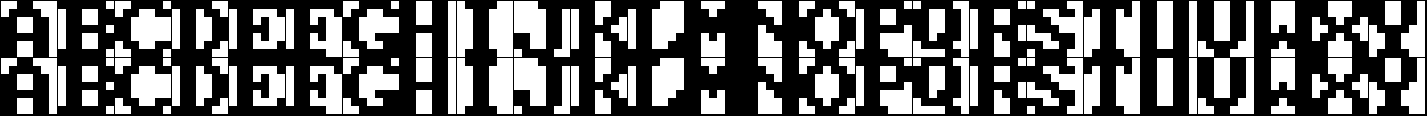
\includegraphics[width=9cm]{fig/im_both.png}
    \caption{Illustrating the 7x7 images that are used as input and output patterns, the first row being the input patterns and the second being the associated output pattern, here illustrated for an autoassociative case, which is used in the initial experimentation.}
\end{figure}

\subsection{Low-level demonstration}
Following is a demonstration of hippocampal model learning, with figures of model output after each learning iteration for chaotic recall and normal recall, i.e. pattern associations. The two first subsets of autoassociative patterns, that is \{A$\rightarrow$A, B$\rightarrow$B\}, and \{C$\rightarrow$C, D$\rightarrow$D\}, are used as training sets in this example.
Furthermore, the hippocampal module is instantiated with the parameter values as outlined above in tables \ref{table:initial_settings} and \ref{table:firing_rates}, a neuronal turnover rate $\tau = 0.04$, and a DG-weighting of $25$. Neuronal turnover is performed between every learnt training set - that is, only once after learning the \{A$\rightarrow$A, B$\rightarrow$B\} associations, before commencing learning of the two next. Here the convergence criteria is set to a static number of training iterations, equal to $15$, while in the experiments, results are generated and analysed for both a dynamic convergence criteria for both learning and stability during recall, as well as for two configurations of $i$ training iterations for convergence and 'stable' recall. Furthermore, the weight matrices are instantiated according to their respective firing rates, with weights being randomly assigned according to Gaussian distributions using the parameters in table \ref{table:initial_weight_distributions}, for a number of neurons corresponding to the layers' firing rates (as outlined in table \ref{table:firing_rates}).

Instantiating the hippocampal model using the parametrization as outlined above, I generated images of the network output for pattern recall (i.e. associations), and chaotic recall for every training iteration. These were generated using both synchronous, and asynchronous updating of the CA3-layer of the model.

\begin{figure}
    \centering
    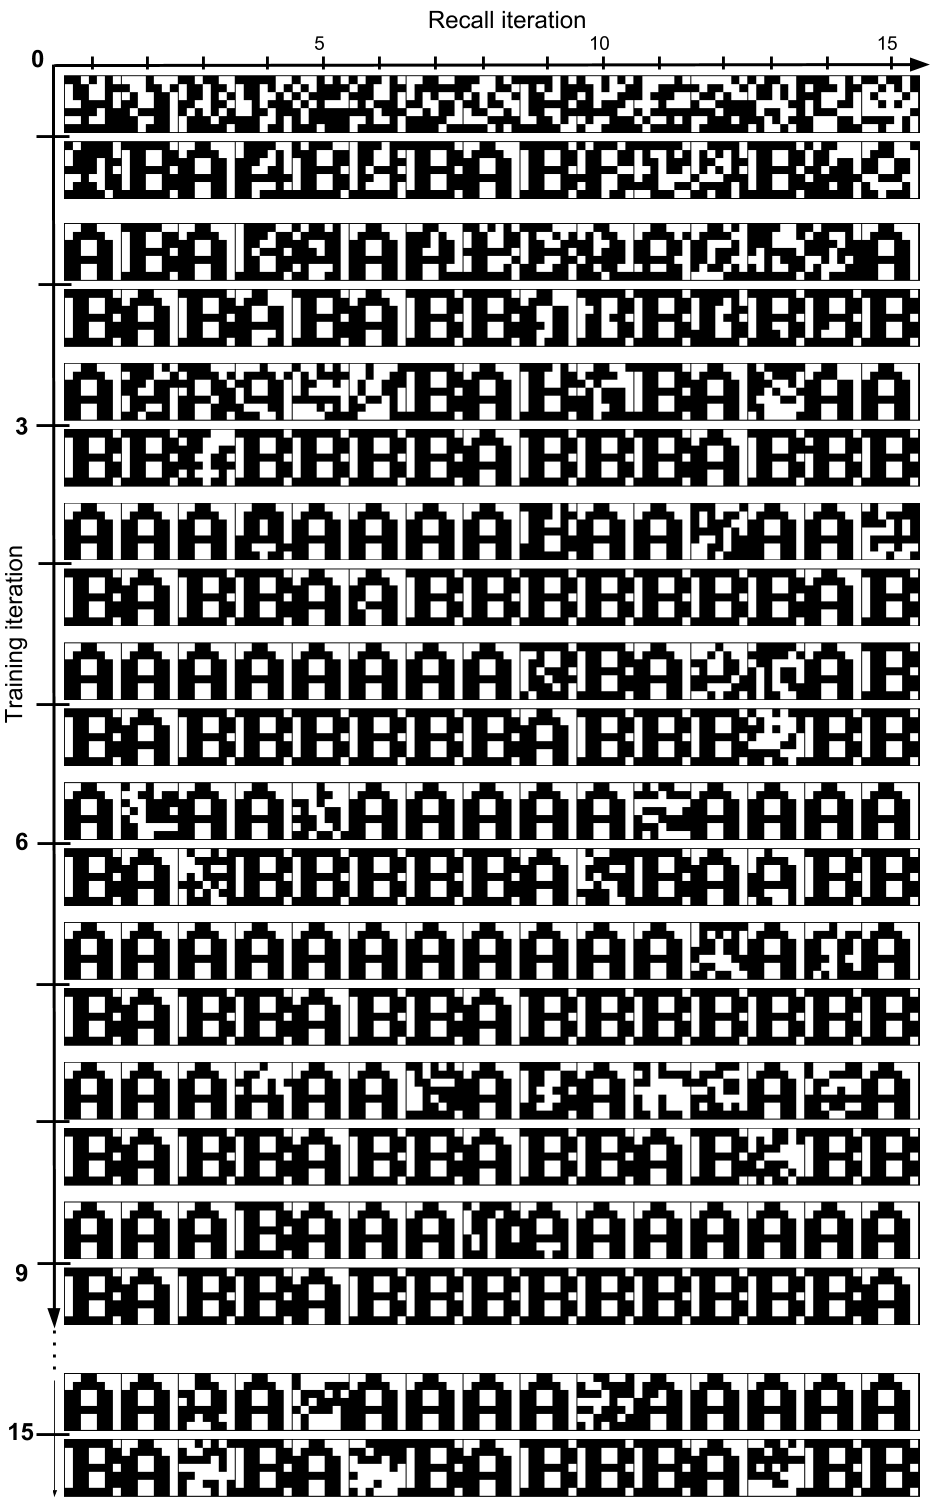
\includegraphics[width=11cm]{fig/AB-pattern-associations-sync-tm0-dgw25}
    \caption{Displaying the recalled pattern for inputs A for the upper row, and B for the lower row, for every learning iteration.}
    \label{fig:pattern_associations_sync}
\end{figure}

\begin{figure}
    \centering
    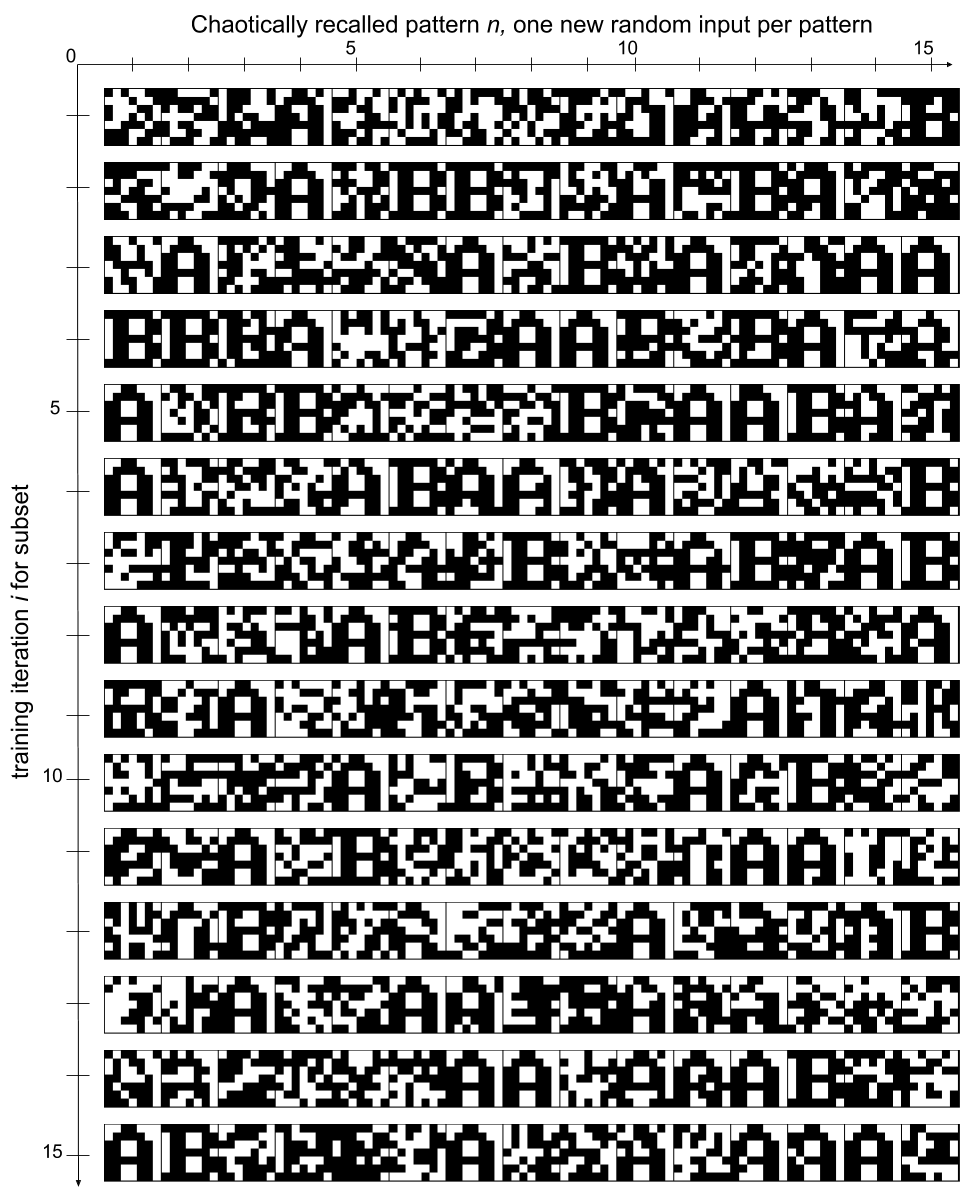
\includegraphics[width=12cm]{fig/AB-chaotic-recall-sync-tm0-dgw25}
    \caption{Displaying the patterns which were recalled by chaotic recall - that is, for each training iteration, 15 patterns were recalled. For each pattern that was recalled, a (new) random input was generated and set as the model's input. Note also that using the same random input also would yield chaotically recalled patterns, which is also included in the trials and experiments contained later in this chapter.}
    \label{fig:chaotic_recall_sync}
\end{figure}

When studying the two figures (\ref{fig:pattern_associations_sync}, \ref{fig:chaotic_recall_sync}) that display the recalled patterns during and after learning pattern-associations for patterns A$\rightarrow$A, and B$\rightarrow$B, note that pattern separation seems fairly successful, as the associated output for aforementioned letters is fairly stable at the corresponding output. However, some spurious patterns appear, even in the case of having the actual, non-distorted input of the pattern as the model's input. This may signal a weak convergence, which may be due to incorrect model calibration, such as too heavy a DG-weighting. Because the connections from the DG-layer are both instantiated rather heavily ($\mu=0.9, \sigma=0.01$), and weighted 25 times stronger than the connections from the EC- and CA3-layer, this may possibly disrupt the strength of the attained basins of attraction, or prolong the training period needed to have the model converge for its EC-CA3, CA3-CA3, and thus CA3-output connections, and thus the basins of CA3-CA3 settle into place. Now, one run is not sufficient to determine whether this is the case. Therefore, these are parameters that will be tested in further experiments, where 20 trials is most commonly used in order to statistically determine patterns of the emergent model behaviour.
Lastly, it is worth noting that although model convergence and recall is fairly good in the case of having a non-distorted training pattern input as input, a great number of spurious patterns are recalled in the chaotic recall scheme. Thus, the number spurious patterns extracted from chaotic recall is one of the measures that will be used in further analyses. Particularly with regards to successful pattern separation and the establishing of basins of attraction. I.e. perfect recall rate may be erroneously observed as close to 100 \% of the training patterns - however, when the number of spurious chaotically recalled patterns exceeds this number by a great deal, the quality of the model performance may still be considered poor. Note, however, that it might be interesting to also consider memory consolidation in such a scheme to the neocortical module. I.e. whether a functional mapping is yet contained in the spuriously recalled patterns - as given random inputs may still determine a functional mapping to a seemingly spurious output. Note that in the case of attaining a spurious pattern output for an input from the training set, the functional mapping is most likely not present, and will only disrupt the convergence in the network which attempts to learn the pattern-associations.

% Furthermore, this instability, or oscillation between the model's basins of attraction, is further demonstrated in the figure of chaotically recalled patterns, which barely recalls the letters A and B, and mostly only spurious patterns that do not resemble the original input nor output patterns. Pattern separation is one of the aspects that are evaluated in this thesis. It is evaluated through successful convergence in the first configurations where the convergence criteria is defined as the output being stable for three iterations of recall. Furthermore, it is analysed in terms of all the configurations by considering the perfect recall rates, as well as spurious pattern recall rates.

In order to demonstrate another hippocampal model configuration, low level results are presented below for the case of asynchronous updating of the CA3-layer. Neuronal turnover is still only performed between the two learning sets, which may be argued to be biologically unrealistic (some recoding of weights, i.e. topological synaptic modification) may be argued to be continuously present, at a low rate. The latter is something that will be addressed in later experiments. Nonetheless, this constructed low level example introduces randomness in its training and recall by non-synchronously updating the neurons of its CA3-layer for each training and recall iteration. This may be considered to be somewhat more realistic biologically speaking, although still implausible in terms of that only one neuron is updated at a time algorithmically - in a true and more biologically realistic mode, all neurons should be updated simultaneously, hard-ware level parallelism determining a random queue of updates, making sub-sets of neurons fire and wire simultaneously. Because activity on the population level is what is considered in this model, as well as for several iterations, I consider the attained results to still yield valid suggestions on the neural network level.

\begin{figure}
    \centering
    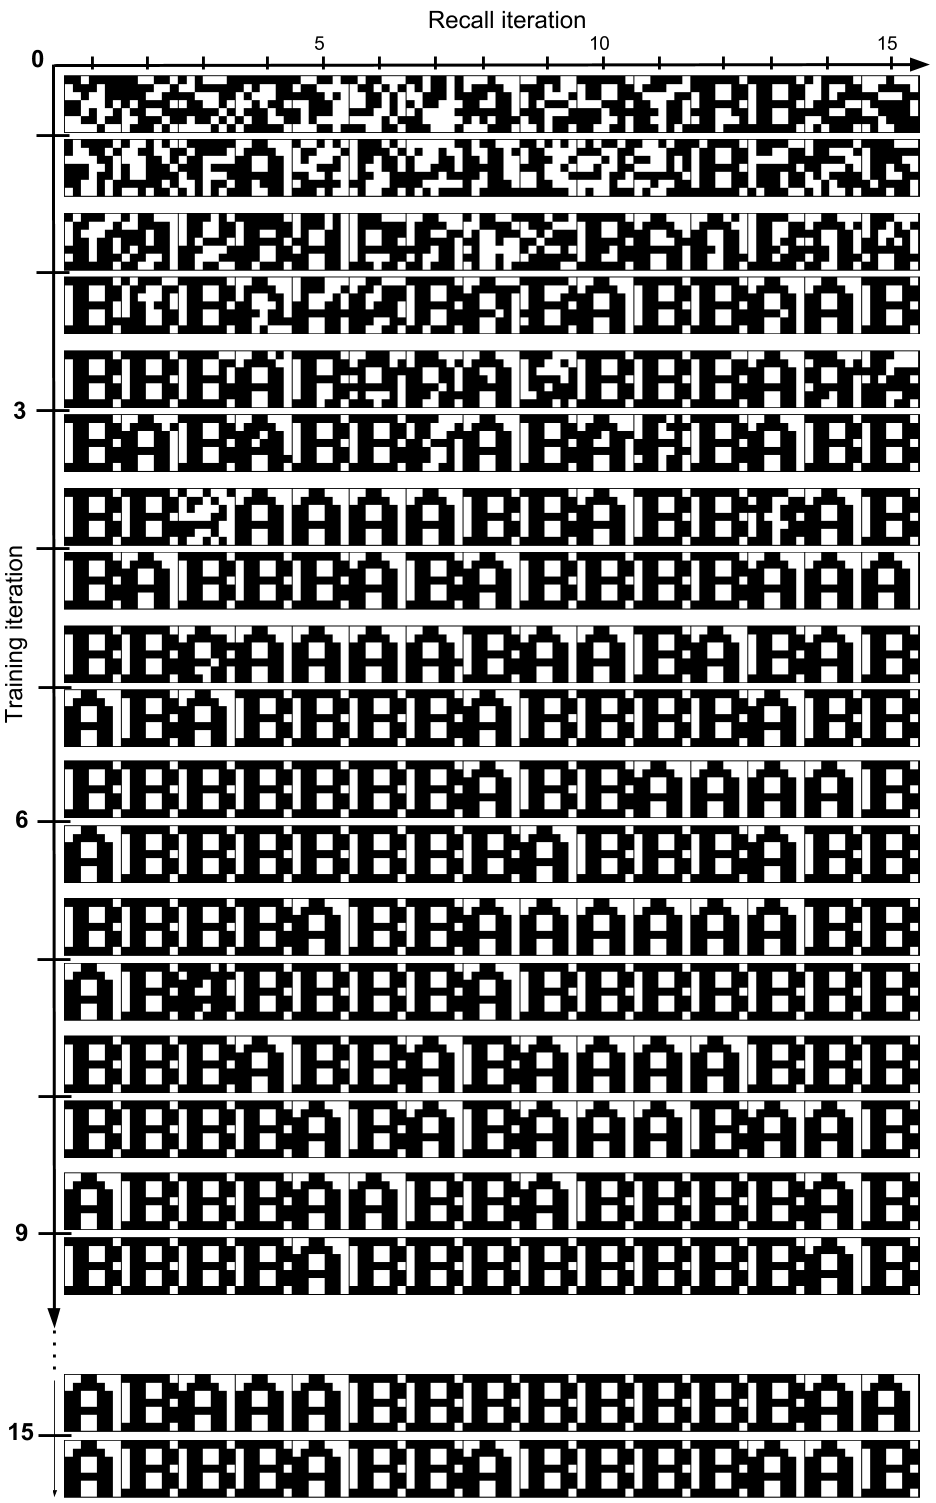
\includegraphics[width=11cm]{fig/AB-pattern-associations-async-tm0-dgw1-tau050}
    \caption{recall. async tm0 dgw1 tau050}
    \label{fig:low-level-3}
\end{figure}

\begin{figure}
    \centering
    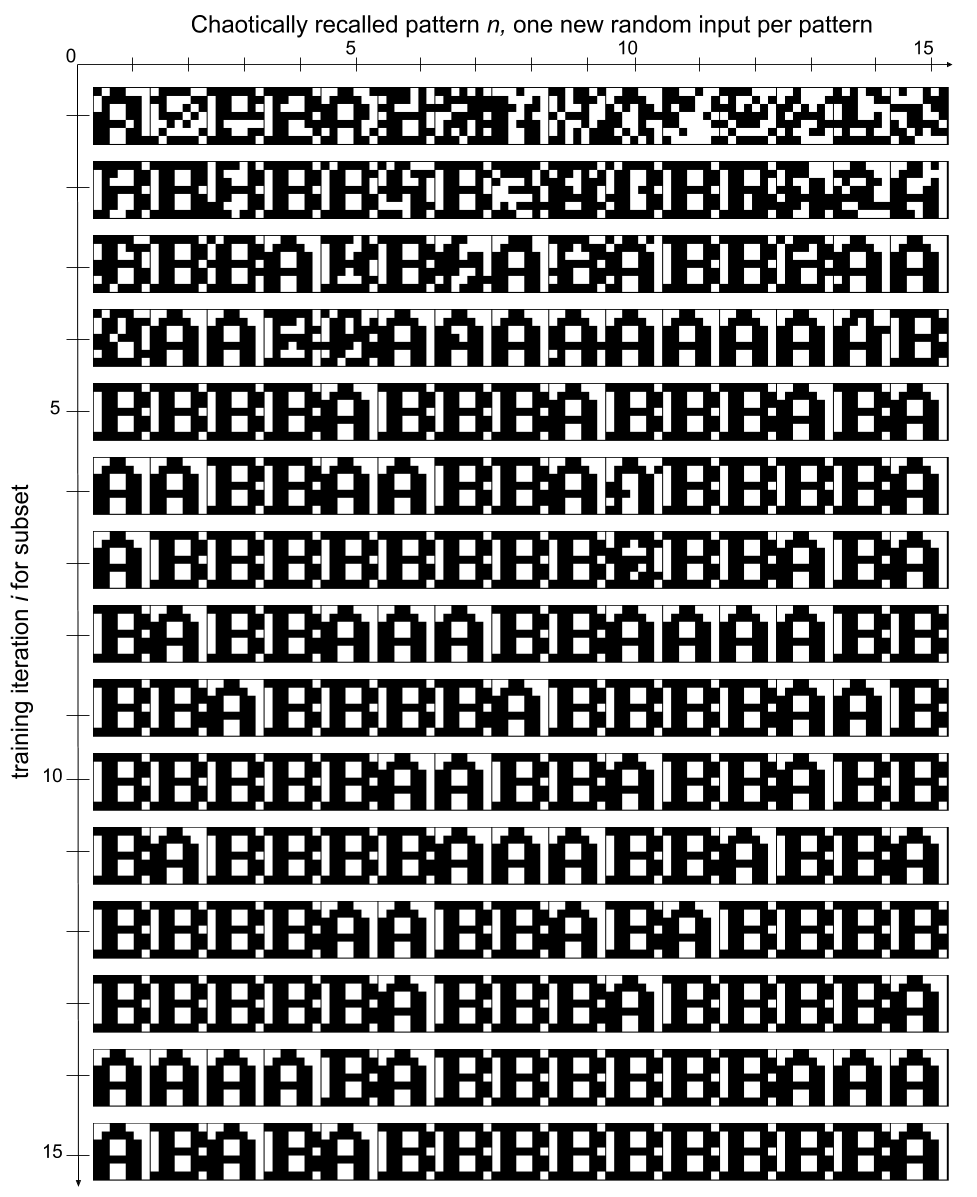
\includegraphics[width=12cm]{fig/AB-chaotic-recall-async-tm0-dgw1-tau050}
    \caption{chaotic recall. async tm0 dgw1 tau050}
    \label{fig:low-level-4}
\end{figure}

Note that while the quality of chaotic recall appears better in figures \ref{fig:low-level-3}, and \ref{fig:low-level-4}, the scheme is less stable for the output for a learnt pattern association's input. This is expected, as more randomness is introduced in the random sequence of updating the neurons of the CA3-layer, which will tend to have the model find the other basin of attraction more easily. Because these results were attained only from one run, the generalisability is somewhat restricted. However, the results do suggest a trend towards a more specific extraction capability at the cost of less stability. It is worth keeping this in mind when considering further experiment results. For the interested reader, the figures presenting the attained output for the next training set, i.e. subset of the training patterns, are contained within appendix E.


\subsection{Experiment 1: Schemes for updating the CA3-layer and performing neuronal turnover}

In order to evaluate the impact of synchronous action potential propagation and synaptic weight modification occurs, four different CA3-layer neuronal activation and weight modification schemes are used. Namely updating the values synchronously, reducing the propagation of values from one layer of neurons to another to a set of vector and matrix operations, or asynchronously, requiring updating each and every neuron independently. In the simplest case of synchronous updating, i.e. for all non-chaotic layers, the synchronous propagation scheme is simply reduced to a vector of activation values multiplied by a weight matrix, which is adjusted through an activation function. For each of these schemes; synchronous or asynchronous updating, two turnover modes are tested. Firstly, turnover is performed only once before every new training subset, i.e. between learnt training sets. Secondly, turnover is performed between every training set iteration, i.e. for every iteration over the current subset.

In this experiment, 20 trials is performed for every full auto-associative training set (that is 2x5, 3x5, 4x5, and 5x5), for every configuration. In other words, 80 experiments are run for each configuration on the model, where the model attempts to learn to associate the for n first capital letters auto-associatively. Furthermore, the convergence criterion is defined as the following: For each training pattern in the current training set, if the model output is the correct pattern output for the undistorted pattern-input for three recall iterations, the pattern is considered to be successfully learnt. If this is the case for every pattern in the current training set, convergence is considered to be attained, and chaotic recall is performed. Chaotic recall is performed similarly to the procedure in \citep{Hattori2010, Hattori2014}. That is, during chaotic recall, when the output remains unchanged for three recall iterations, the pattern is considered learned and chaotically recalled. This is performed for 300 time-steps, with the input to the network being a new random input once a pattern has been (chaotically) extracted.

% \begin{figure}
%     \centering
%     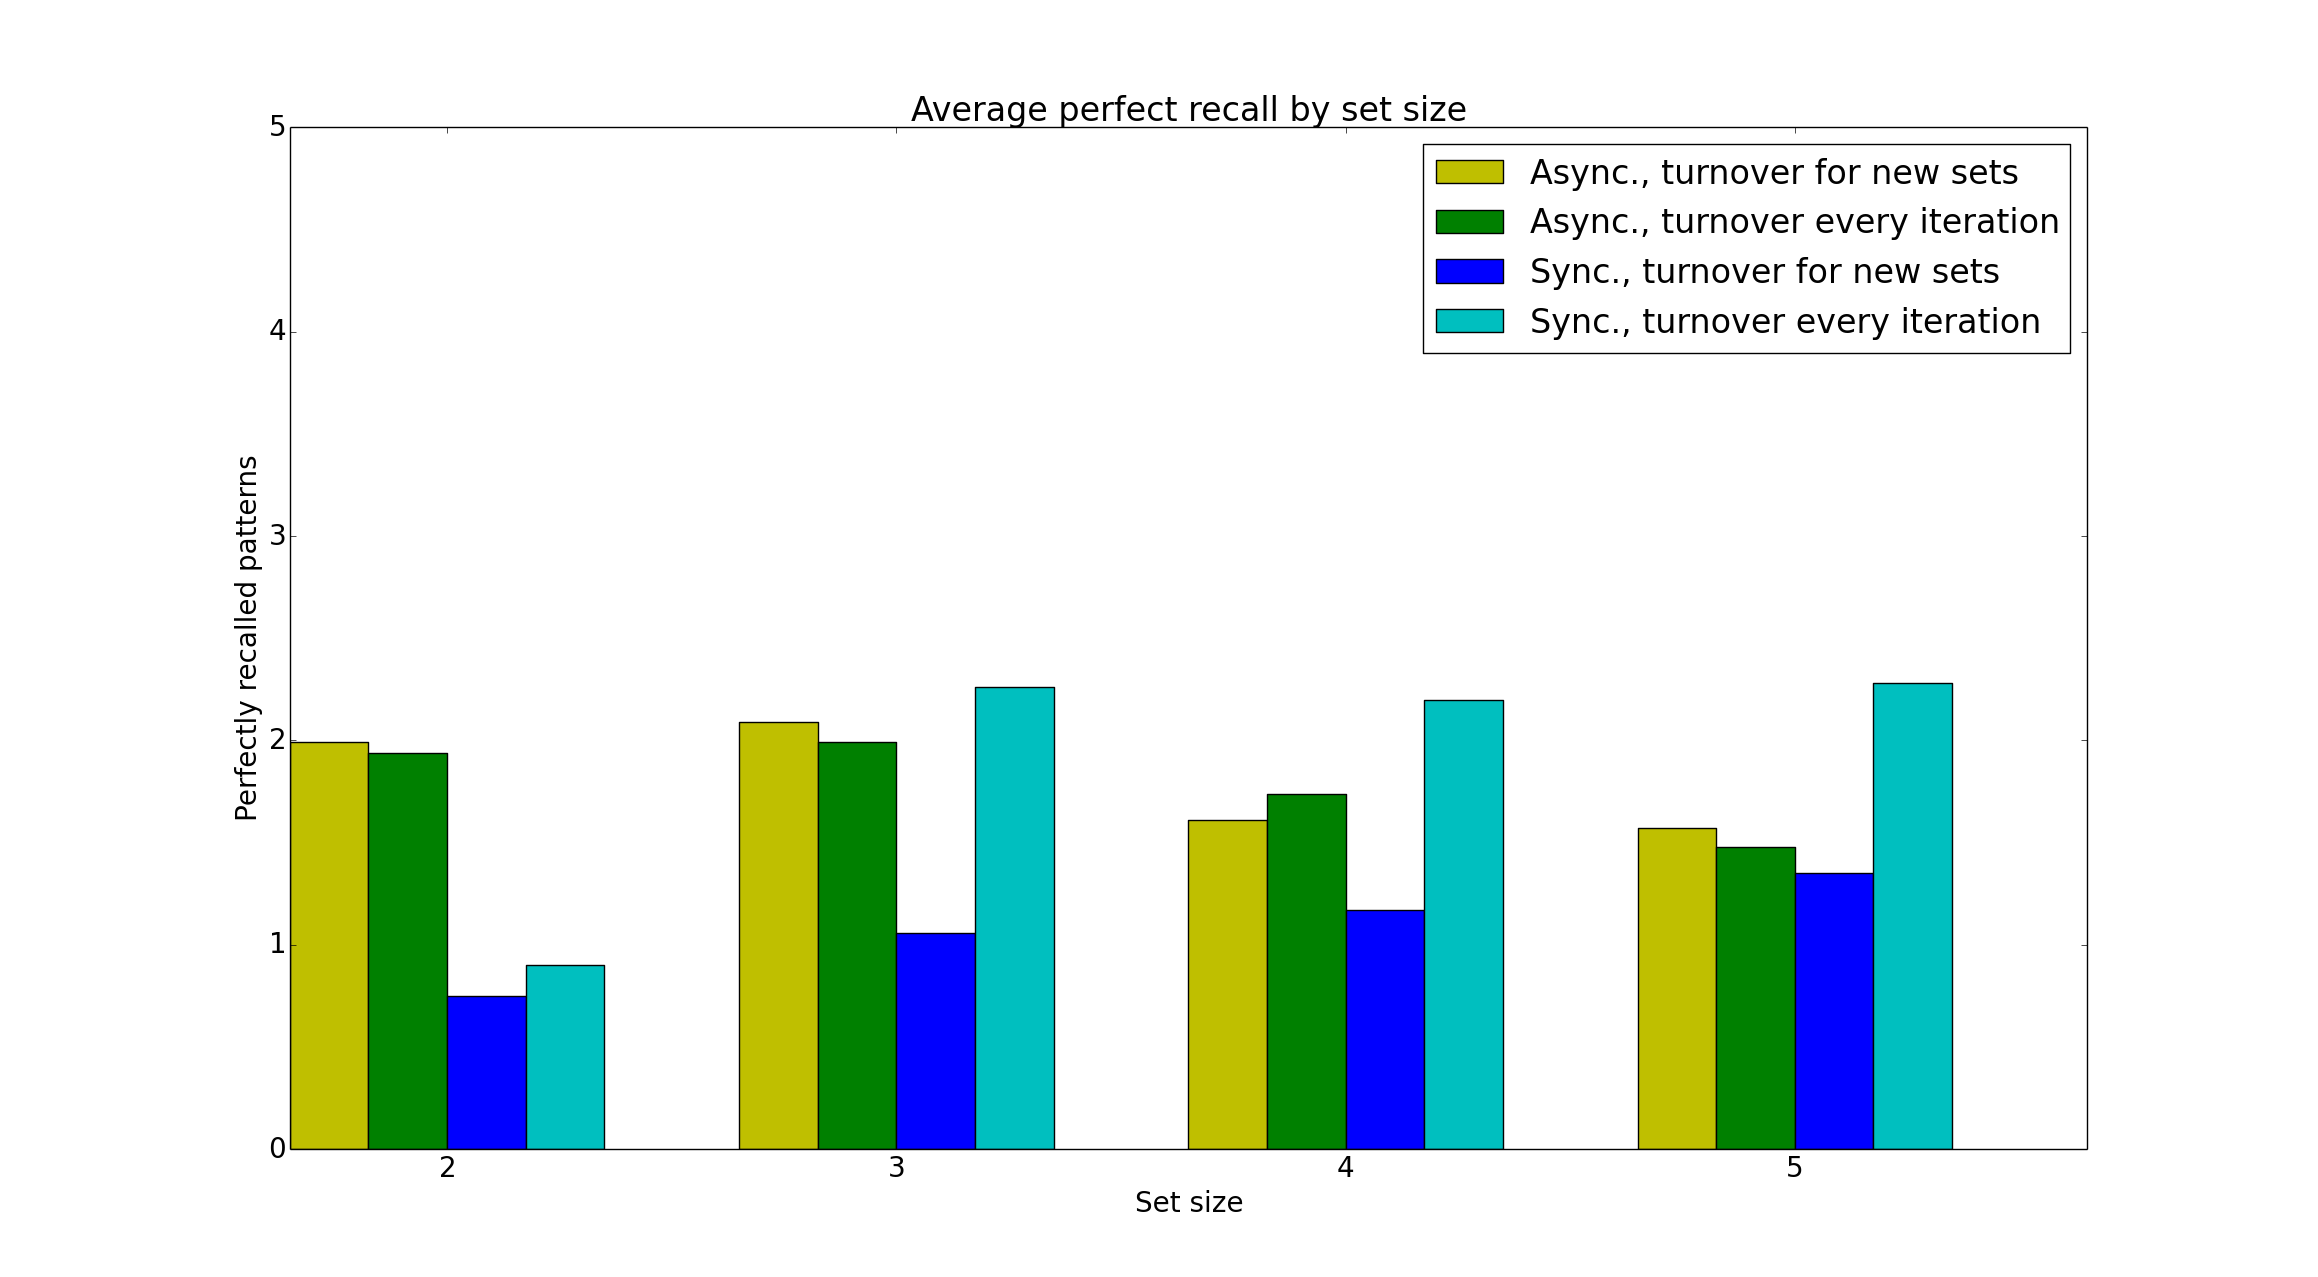
\includegraphics[width=14cm]{fig/average_perfect_recall_rates_by_set_size_bars_reset_for_every_experiment}
%     \caption{Displaying the average number of perfectly recalled patterns by set size for the four different model configurations. Note that the dentate gyrus weighting is set to 25, and the turnover rate to $0.50$ in all of the configurations, which might impact particularly the turnover mode in which turnover is performed between every training iteration.}
%     \label{fig:avg_perfect_recall_bars}
% \end{figure}

\begin{figure}
    \centering
    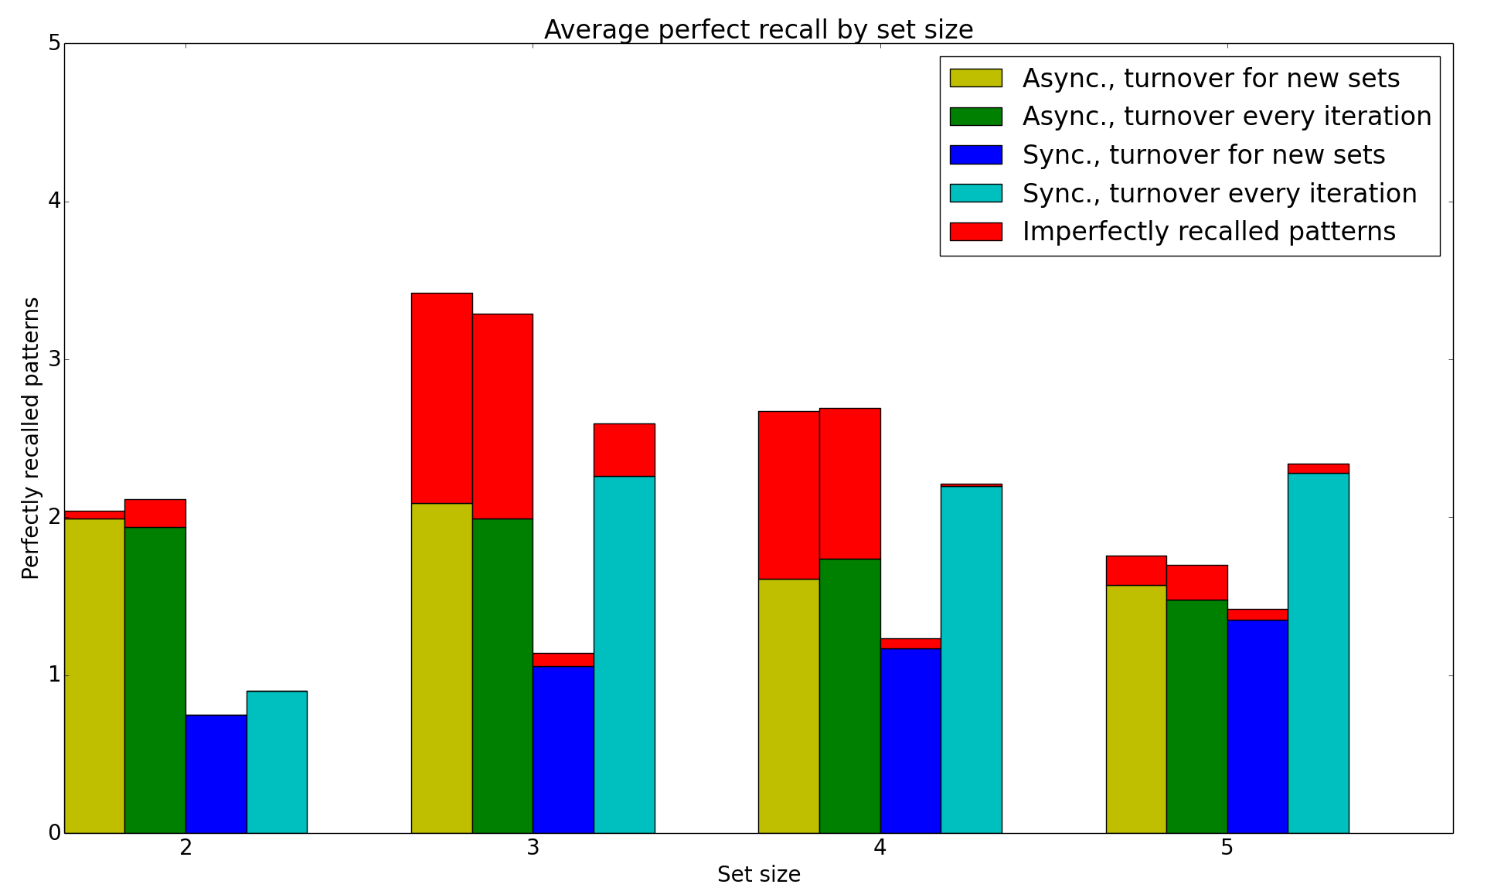
\includegraphics[width=13cm]{fig/cut_prr_with_spurious_reset_every_experiment}
    \caption{Displaying the average number of perfectly recalled patterns for each mode configuration, along with the average number of spuriously recalled patterns for each configuration. Note that the dentate gyrus weighting is set to 25, and the turnover rate to $0.50$ in all of the configurations, which might impact particularly the turnover mode in which turnover is performed between every training iteration.}
    \label{fig:avg_perfect_recall_rates_with_spurious_bars}
\end{figure}

Note that spurious is defined as any distinct non-perfectly recalled pattern in figure \ref{fig:avg_perfect_recall_rates_with_spurious_bars}. Note that in contrast to the introductory examples where the convergence criterion was defined as training or recalling for a fixed number of iterations \textit{i}, (\textit{i} $=15$ in the introductory low-level examples), having a stricter convergence criterion naturally resulted in no spurious patterns being recalled in the synchronous updating schemes, as may be expected when considering figure \ref{fig:chaotic_recall_sync}. However, it remains unclear whether convergence is attained only from this figure. Therefore, the convergence rate is also logged and presented in figure \ref{fig:convergence_rates_async_sync}.

\begin{figure}
    \centering
    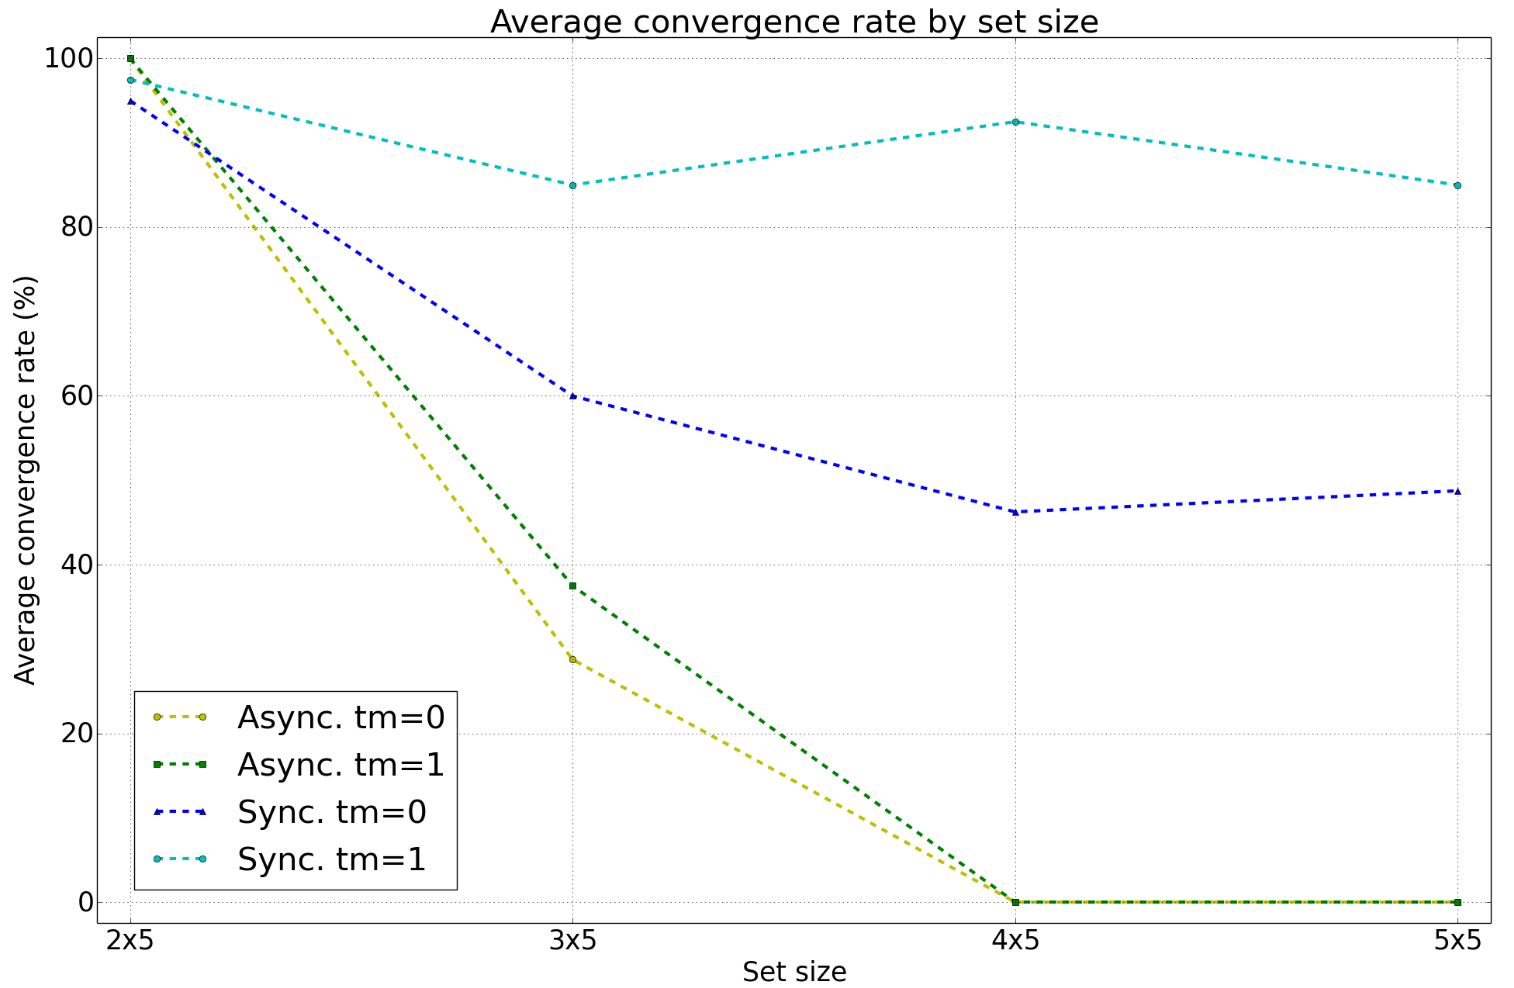
\includegraphics[width=13cm]{fig/avg_convergence_rate_cut}
    \caption{Presenting the average convergence rate in the four experiment-schemes, using the strict convergence criterion. Note that the synchronous updating schemes seem to converge just as well in nearly all cases, except for in the case of set size 5.   [should increase line thickness, include grid too]}
    \label{fig:convergence_rates_async_sync}
\end{figure}

Although extraction of all patterns using chaotic recall is unsuccessful in nearly all schemes, the synchronous schemes converge well for all set sizes, apart from when using turnover for every set iteration for the largest set size (5x5). It is worth emphasizing that the scheme with the best convergence rate converges for nearly 100 \% of the training subsets for all set sizes. However, it is the scheme which performs the worst in terms of perfect recall, i.e. synchronous CA3-layer neuronal updating performing neuronal turnover only between learnt subsets. Furthermore, this scheme recalls nearly no other than 1-2 of the patterns from each training subset, which it recalls perfectly. Demonstrating that while the scheme is likely to successfully be able to separate patterns during training, it does not separate them well enough to be able to chaotically recall them.
Some hypotheses on why training is successful in nearly all cases, but not extraction through chaotic recall, include the following:
- It may simply be that the model adjusts its weights too heavily towards the present firing patterns. However, this hypothesis remains implausible as the convergence criterion ensures that the model is fairly stable for every pattern in the training subset, i.e. the output remains correct for three recall iterations when the corresponding input of the pattern is presented to the network. This is the case in nearly 100 \% of the training cases, unaffected by set size.
- Because every neuron of the CA3-layer is updated synchronously, the model lacks 'jiggle' during recall, making it prone to being stuck in a subset of its basins of attraction. This view is further strengthened by considering that the DG-layer is not used during recall, as it performs expansion encoding, which along with its sparsity may recode and separate similar inputs into separate patterns for the CA3-layer to handle. Because convergence is attained during training, but not recall, this suggests that the DG-layer may in fact give rise to these emergent qualities.
- Another view, which of course may very possibly be intertwined with the former is that
Note that due to the quick convergence qualities of the hippocampal module, it is unlikely that the EC to CA3 connections, as well as the CA3-CA3 connections have not been able to converge towards the solution. However, if the recoding does not settle into a steady pattern, changing the input to the CA3-layer significantly for every training iteration, it may of course be the case that the weights do not converge. This theoretical scenario, however, is even more unlikely to occur, as k-WTA will strengthen the connection weights to the first k winners, thus tending to favor the initial winners for the same input, only changing the output which it projects to the CA3-layer very little, if at all. 
This is exactly the reason for why neuronal turnover is performed - to recode the weight configuration such that the resulting k winners will vary slightly more, thus furthering its recoding abilities, improving pattern separation and model performance. Note that it is the expansion encoding and sparsity in the DG-layer that recodes and separate similar, but distinct patterns. Together with the input of the EC-layer, the current values of the CA3-layer results in updating of weights for the recurrent connection to the layer itself, as well as backwards through the DG- and EC-layer, which again are adjusted according to the 'observed' input for the current pattern. In other words, we seek a configuration for which the model dynamically separates patterns due to its recoding qualities, and yet is able to recall them without the use of the pathways which expand, recode and project its values which separates the patterns. It may be argued that completely omitting this layer during recall is somewhat unrealistic. However, according to physiological findings, this pathway is used very little during recall \citep{Wakagi2008}. Furthermore, due to the auto-associative nature of the CA3-layer, if this layer has successfully converged for patterns with little overlap, it is likely to fall into a basin of attraction, performing pattern completion for partial pattern input. Now, one may think that the EC-layer will not necessarily project a partial, recoded pattern to the CA3-layer, as this recoding is performed in synergy with the DG-layer. However, as the observant reader may have noticed, it is exactly that; in \textit{synergy} with the DG-layer. As recoding has already been performed, this recoding is propagated to all layers of the network model by Hebbian learning. In other words, the synaptic weight modification between the EC-layer and CA3 will reflect the recoded pattern.
Lastly, the nature of the CA3-neurons, i.e. chaotic neurons, may also impact the chaotic recall capabilities of the model. While it appears evident that the zeta- and eta-equations do not limit successful training of patterns, it may be that they impact the next activation values of the CA3-layer too heavily during recall. This may be argued by considering that in the current implementation, the next eta- and thus zeta-values are based on the former eta- and zeta-values along with the sum of the raw input sum, i.e. the sum of the dot products between the anteceding layers' activation value vectors and their corresponding weight matrices, without computing the values' transfer function values. )This may be tested by performing the entire experimental suite using). However, as damping factors are used, the former values will be disregarded at an exponential pace. Leaving only the possibility that the sum of the former values along with the new input sum enhances the gravity of the current basin of attraction. This is unlikely, as the model attains successful convergence for an additional term in the input equation during training, namely the dot product from the DG-layer. Furthermore, this product may be multiplied by a factor up to 25. If anything, this suggests that the eta- and zeta-functions are not at all excited about the DG-layers absence, possibly resulting in its stable mood.


% ========================== RESULTS ============================
\section{Results}

% ========= for all ==========
\begin{figure}[h!]
    \centering
    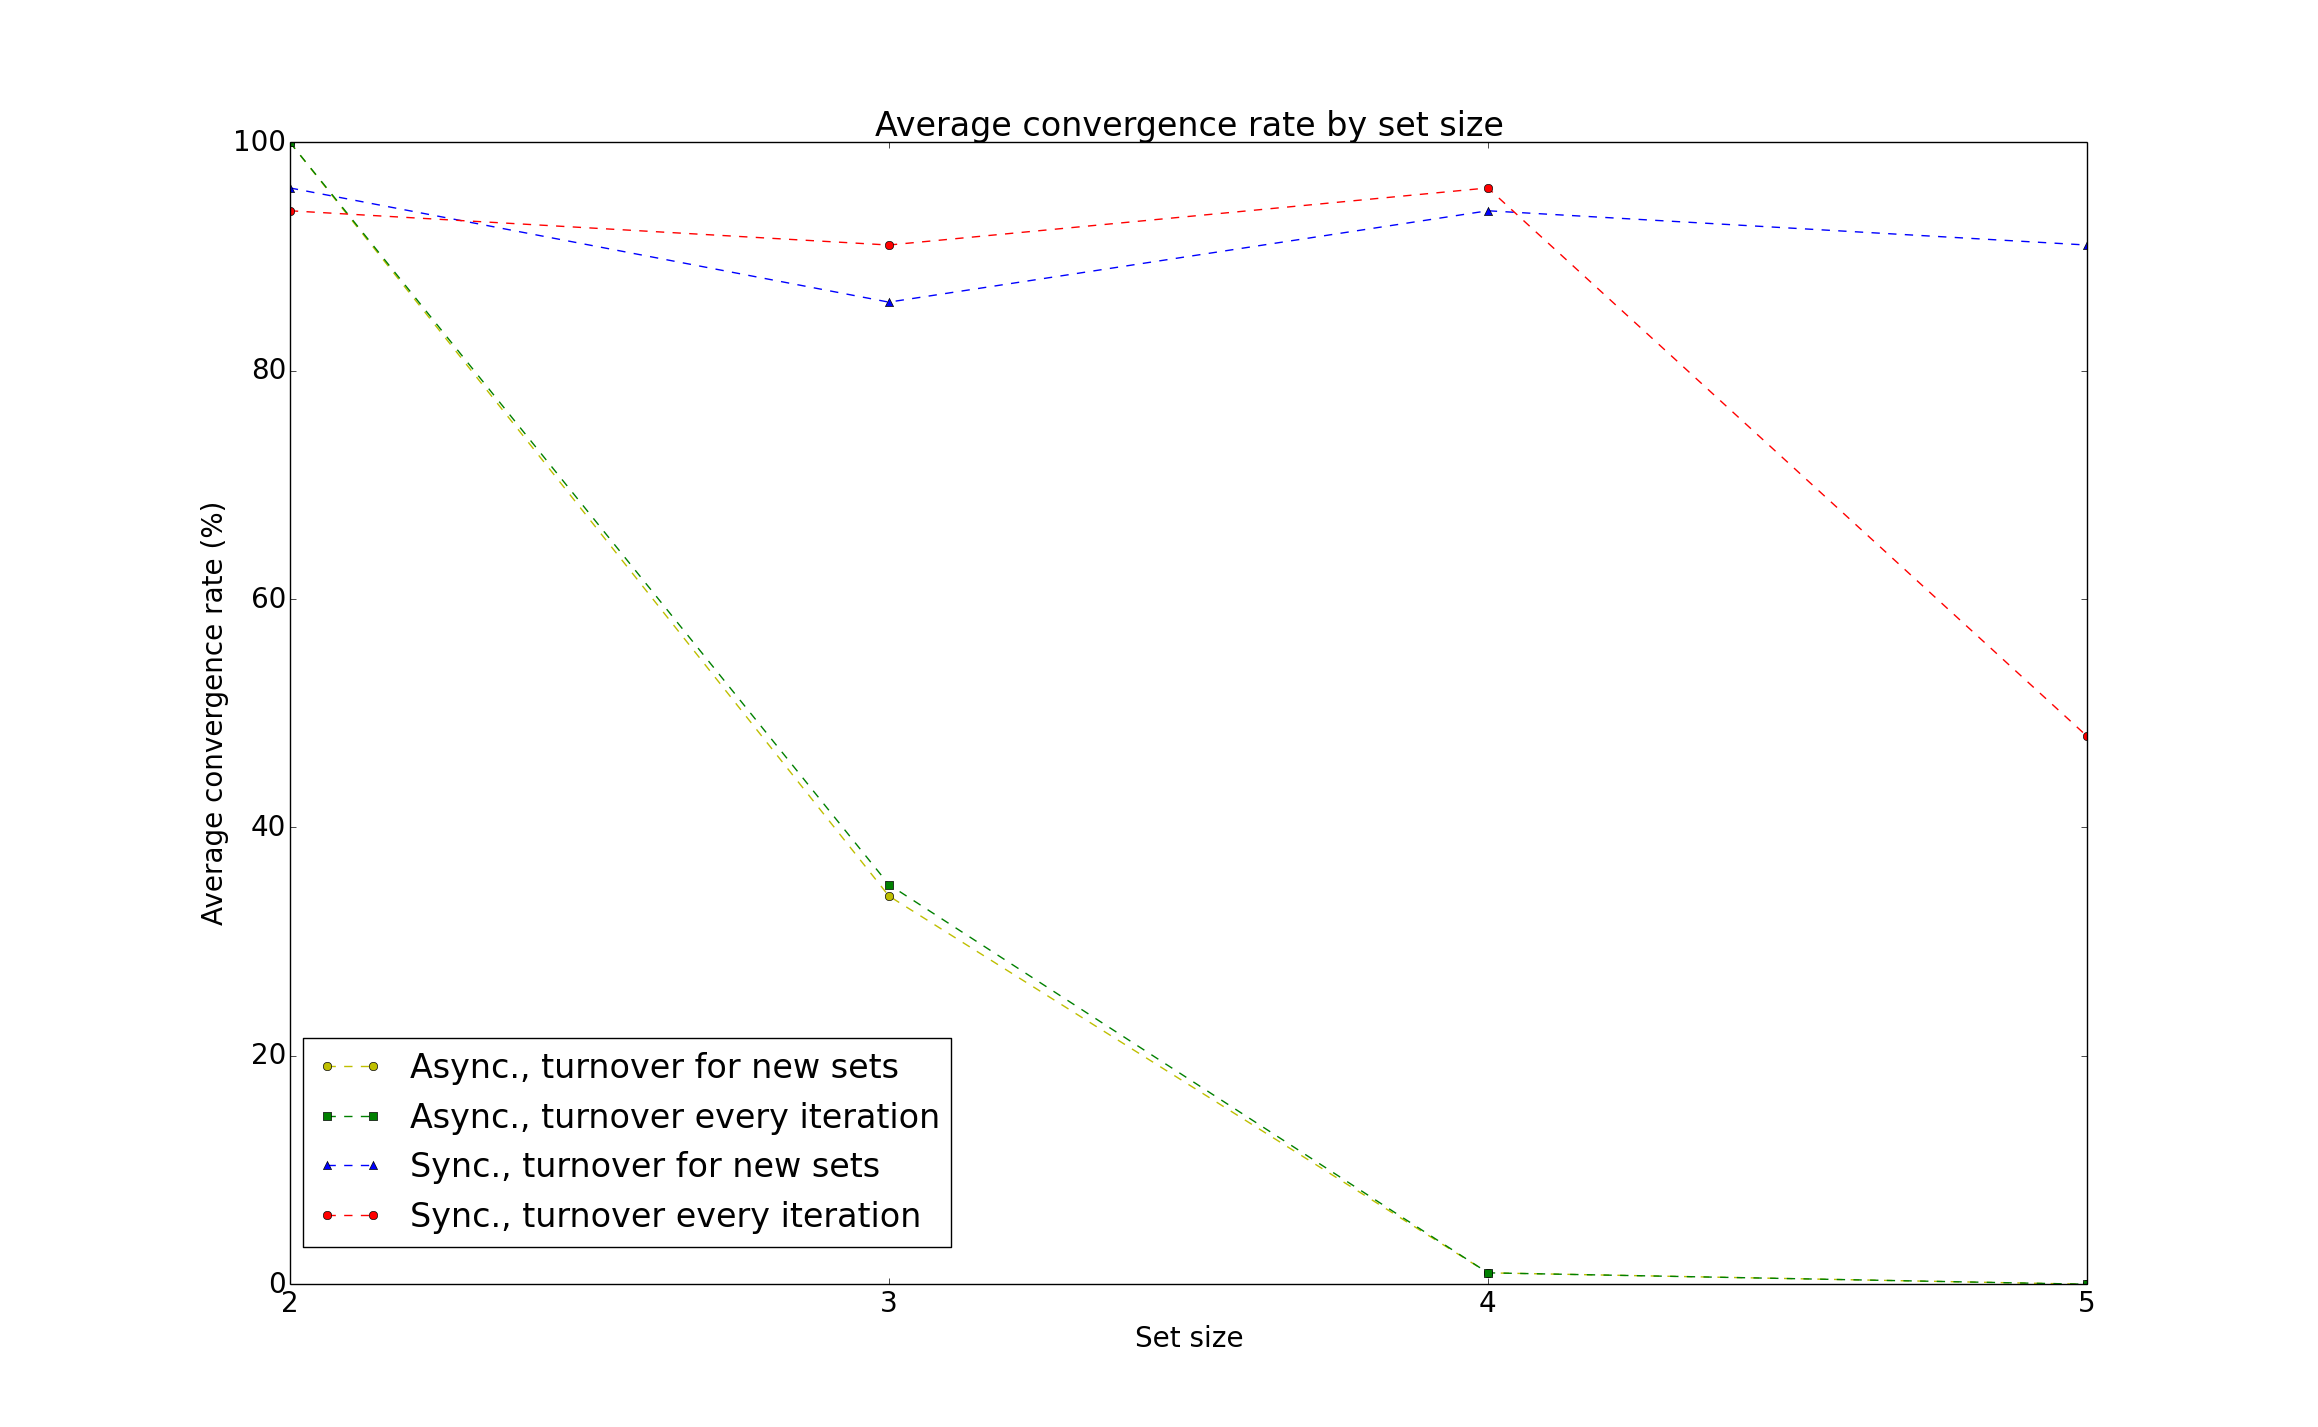
\includegraphics[width=14cm]{fig/avg_convergence_rate.png}
    \caption{avg convergence by set size, dentate gyrus weighting 25, turnover rate $0.5$.}
    \label{fig:avg_convergence_rate}
\end{figure}

\begin{figure}[h!]
    \centering
    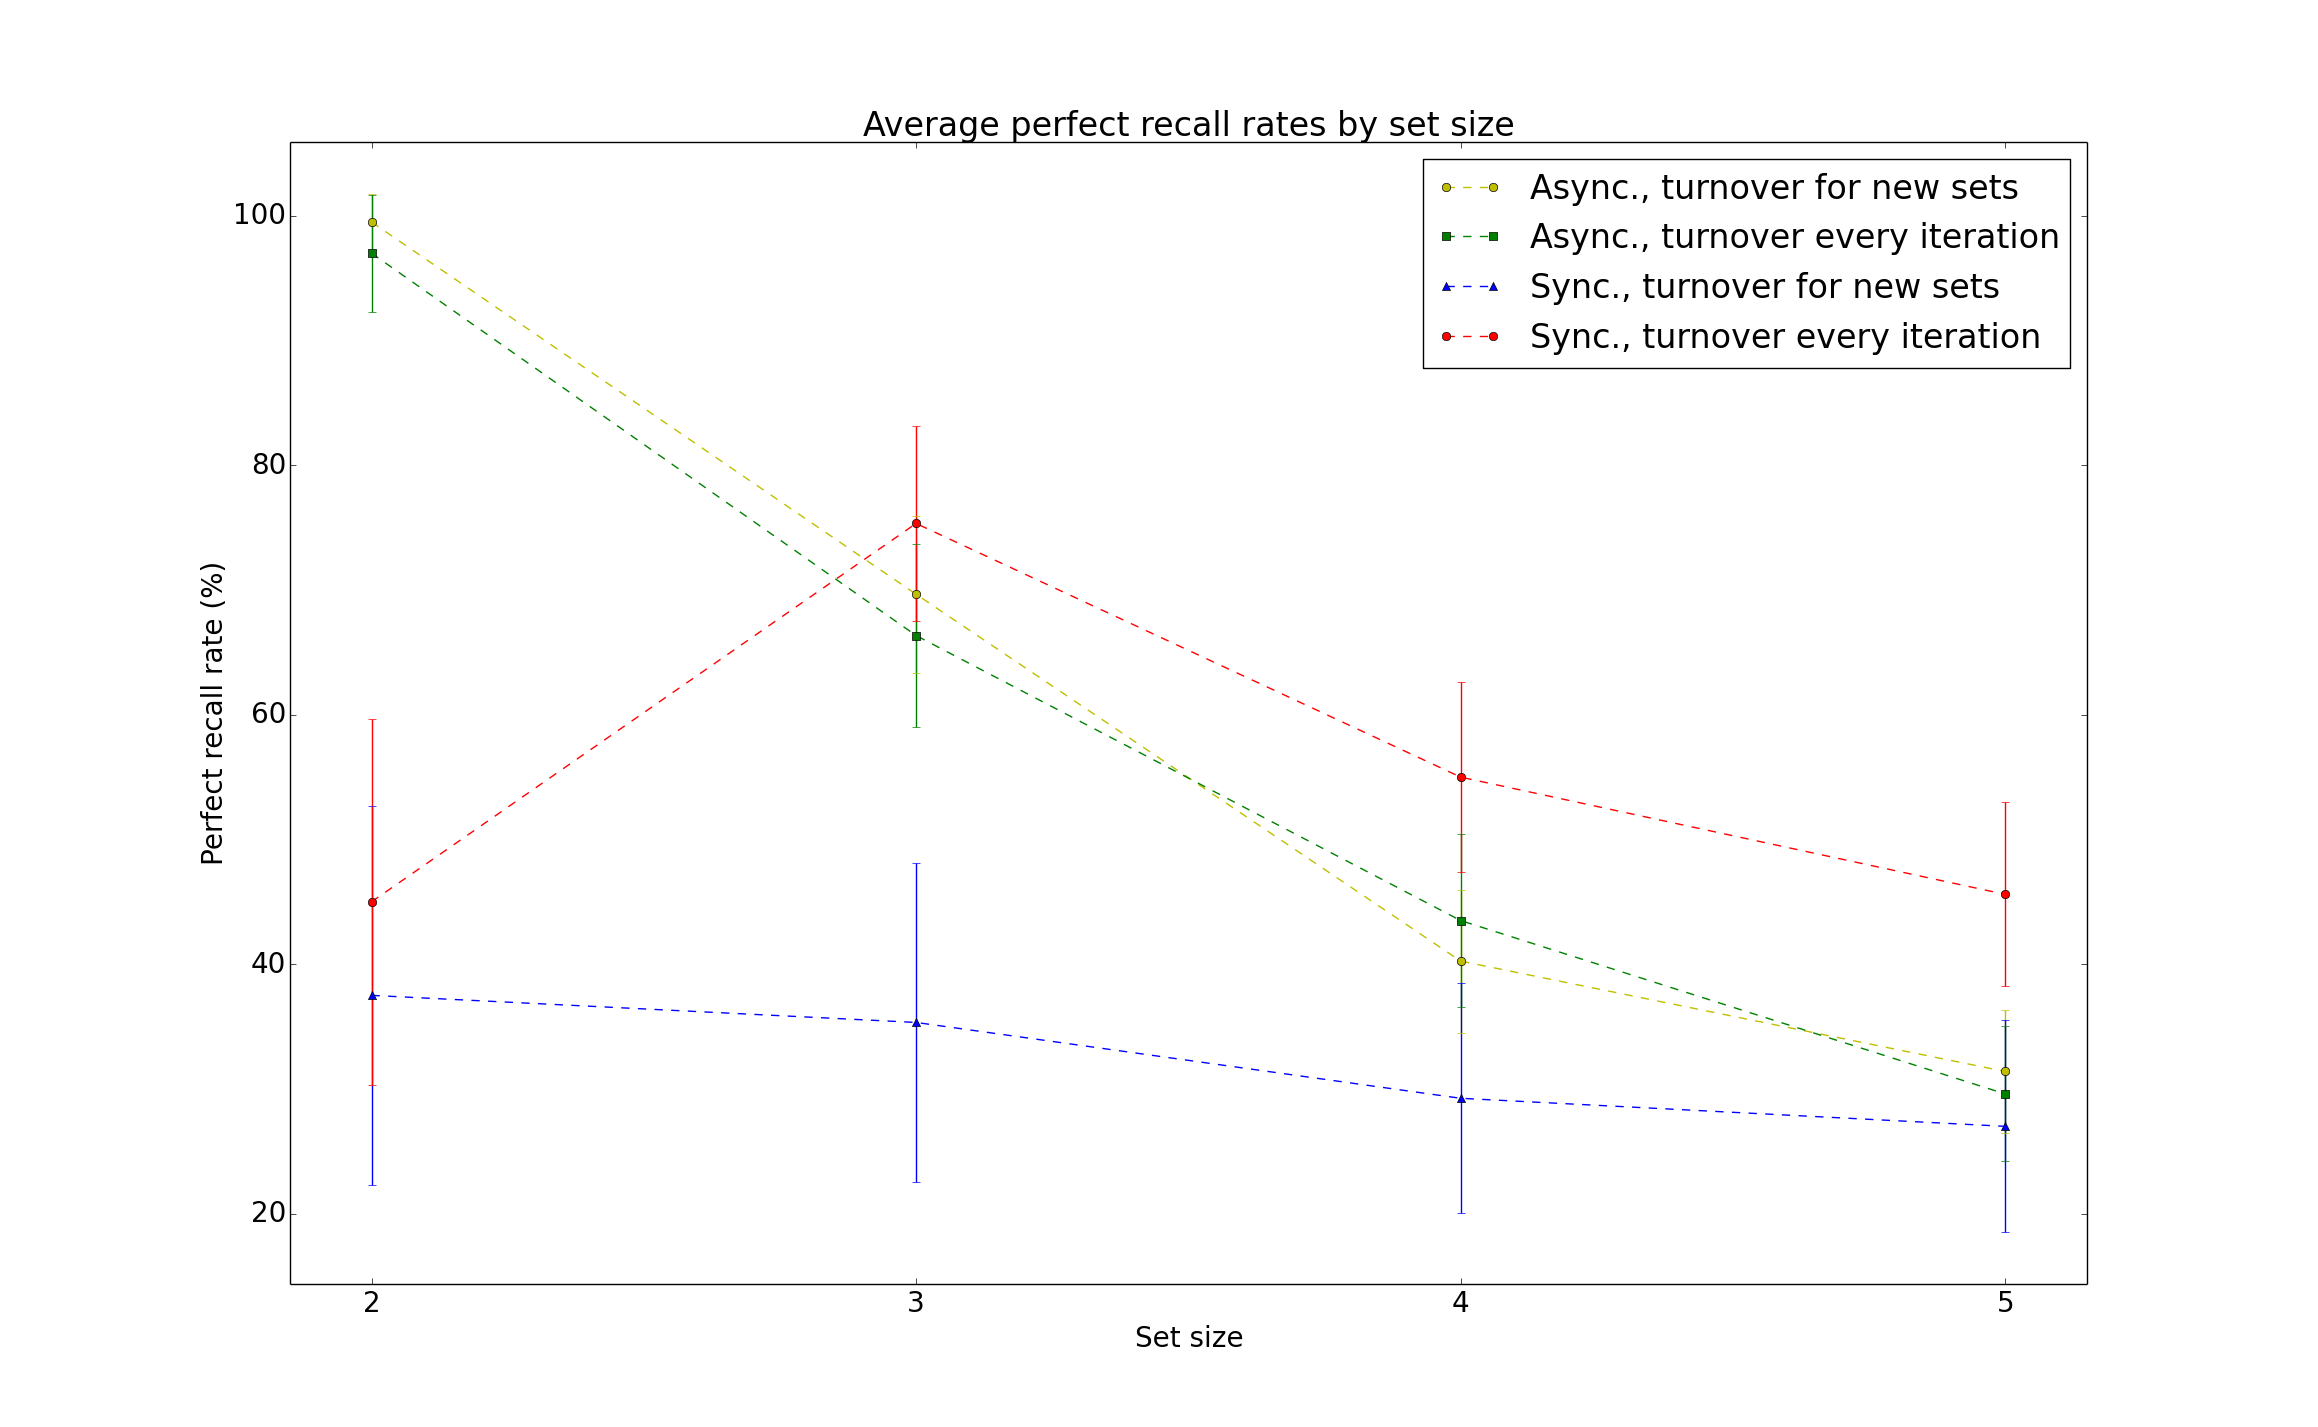
\includegraphics[width=14cm]{fig/avg_perfect_recall_rates.png}
    \caption{perf recall by set size, dentate gyrus weighting 25, turnover rate $0.5$.}
    \label{fig:avg_perfect_recall_rates}
\end{figure}

% \begin{figure}[h!]
%     \centering
%     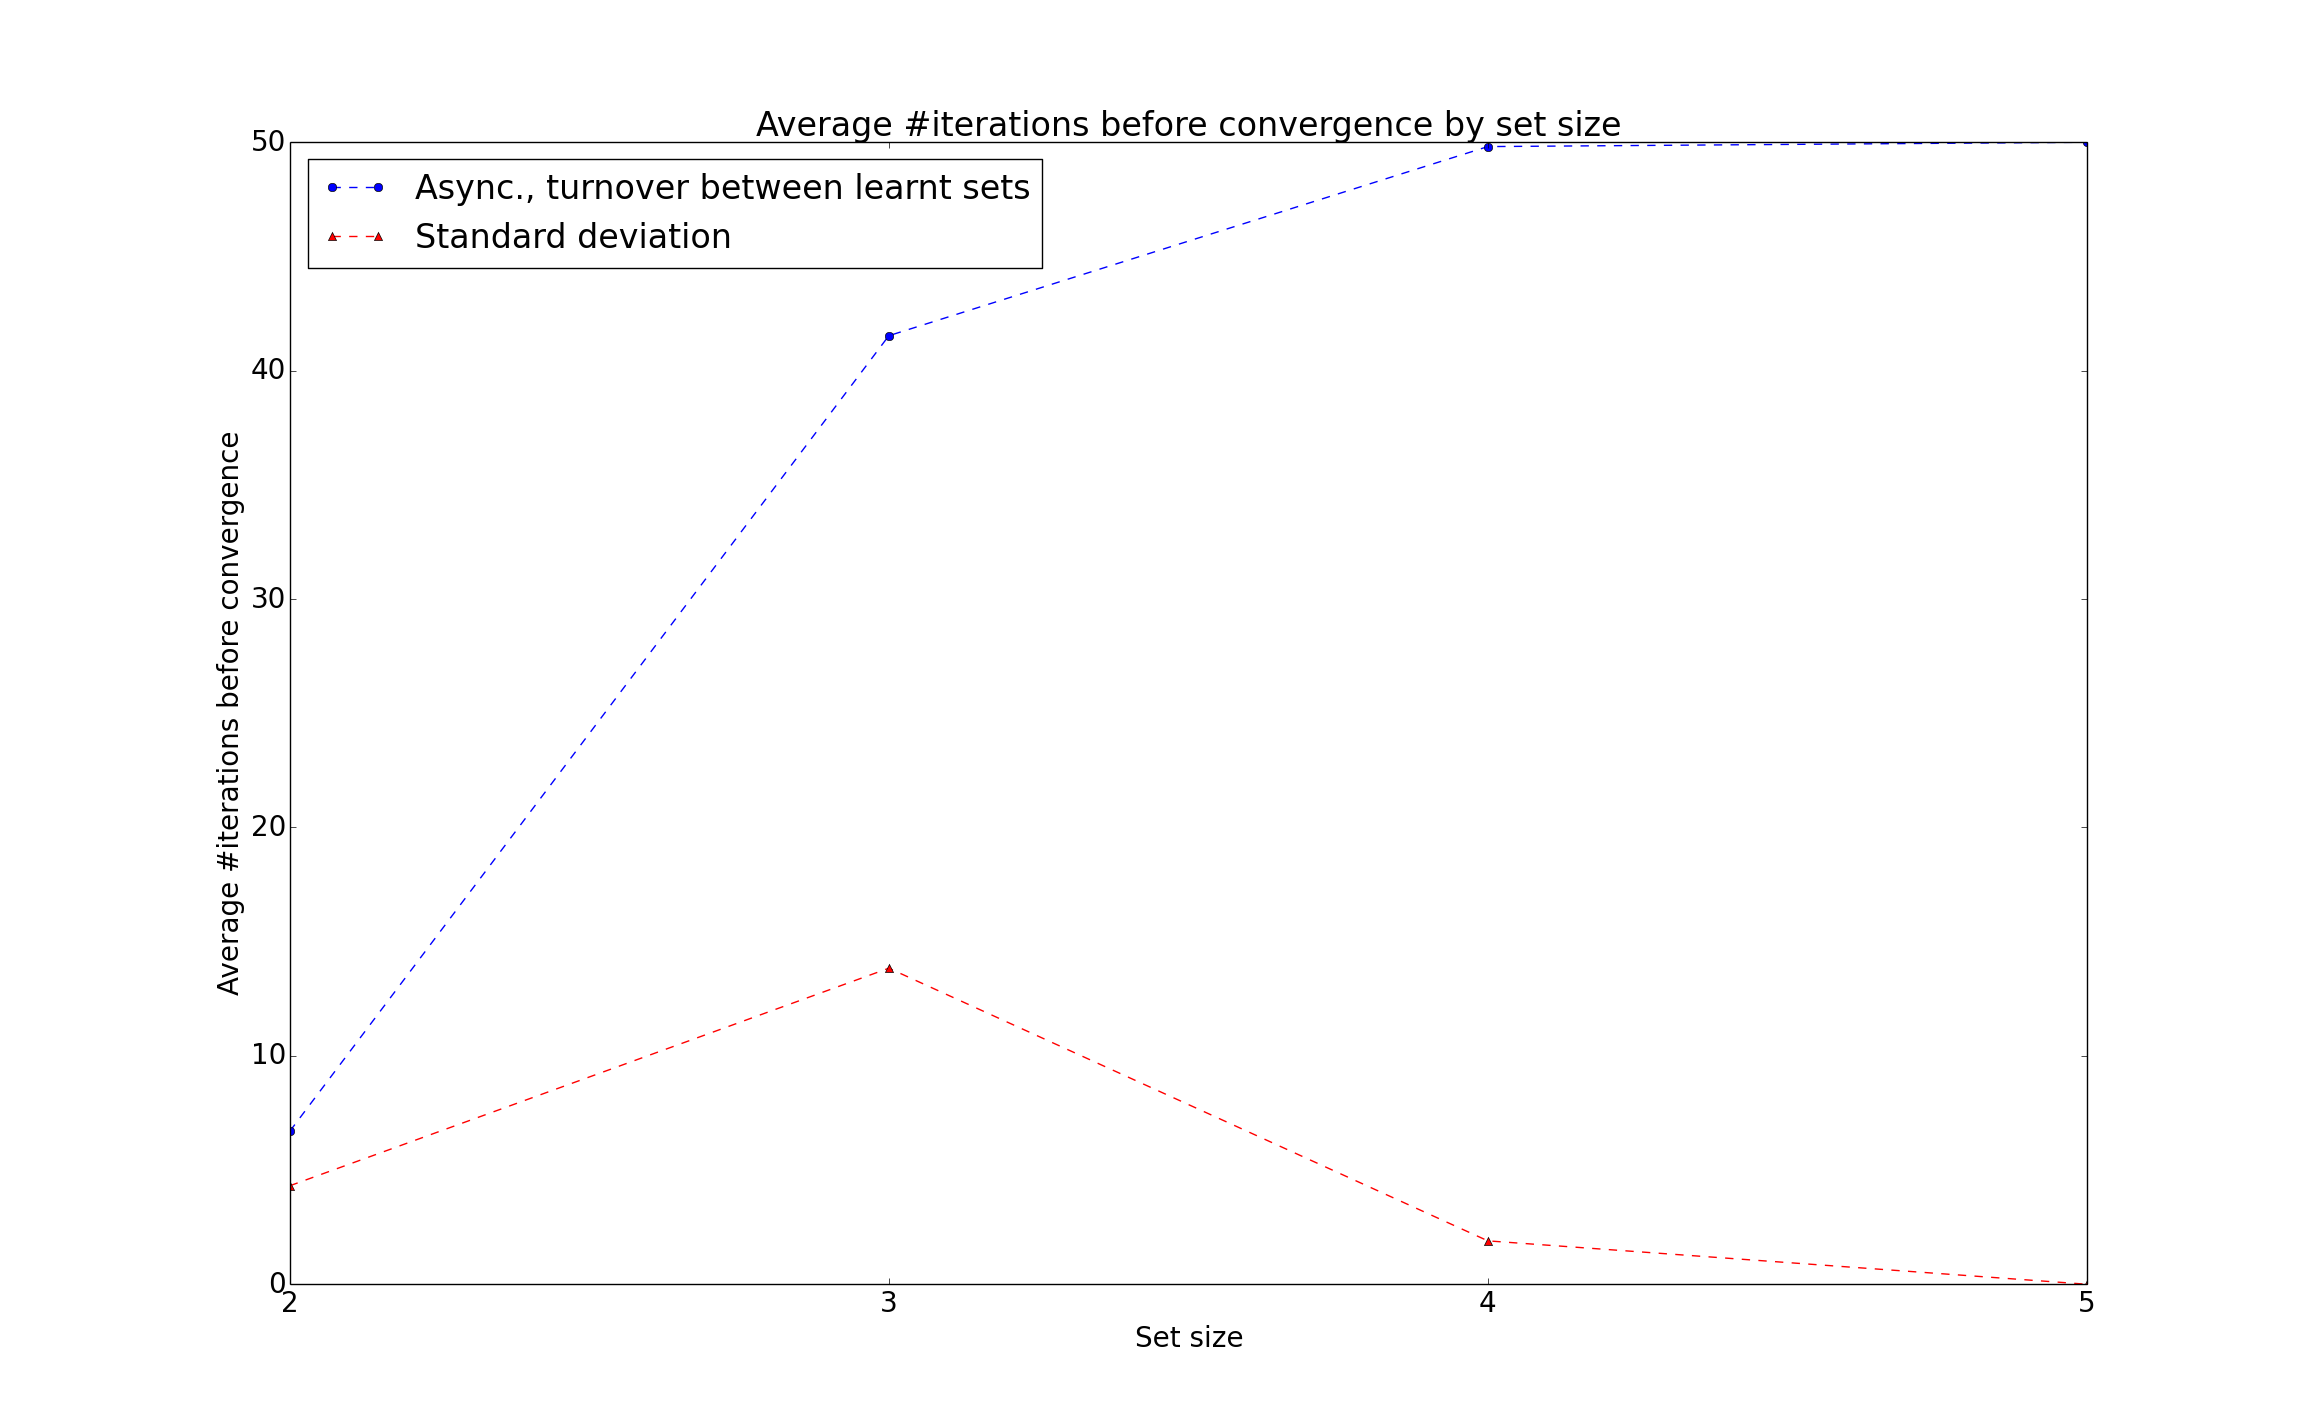
\includegraphics[width=13cm]{fig/avg_convergence_iterations_async_true_mode_0.png}
%     \caption{avg iters to convergence, most successful; async true mode 0}
%     \label{fig:avg_convergence_iterations_async_true_mode_0}
% \end{figure}

% \begin{figure}[h!]
%     \centering
%     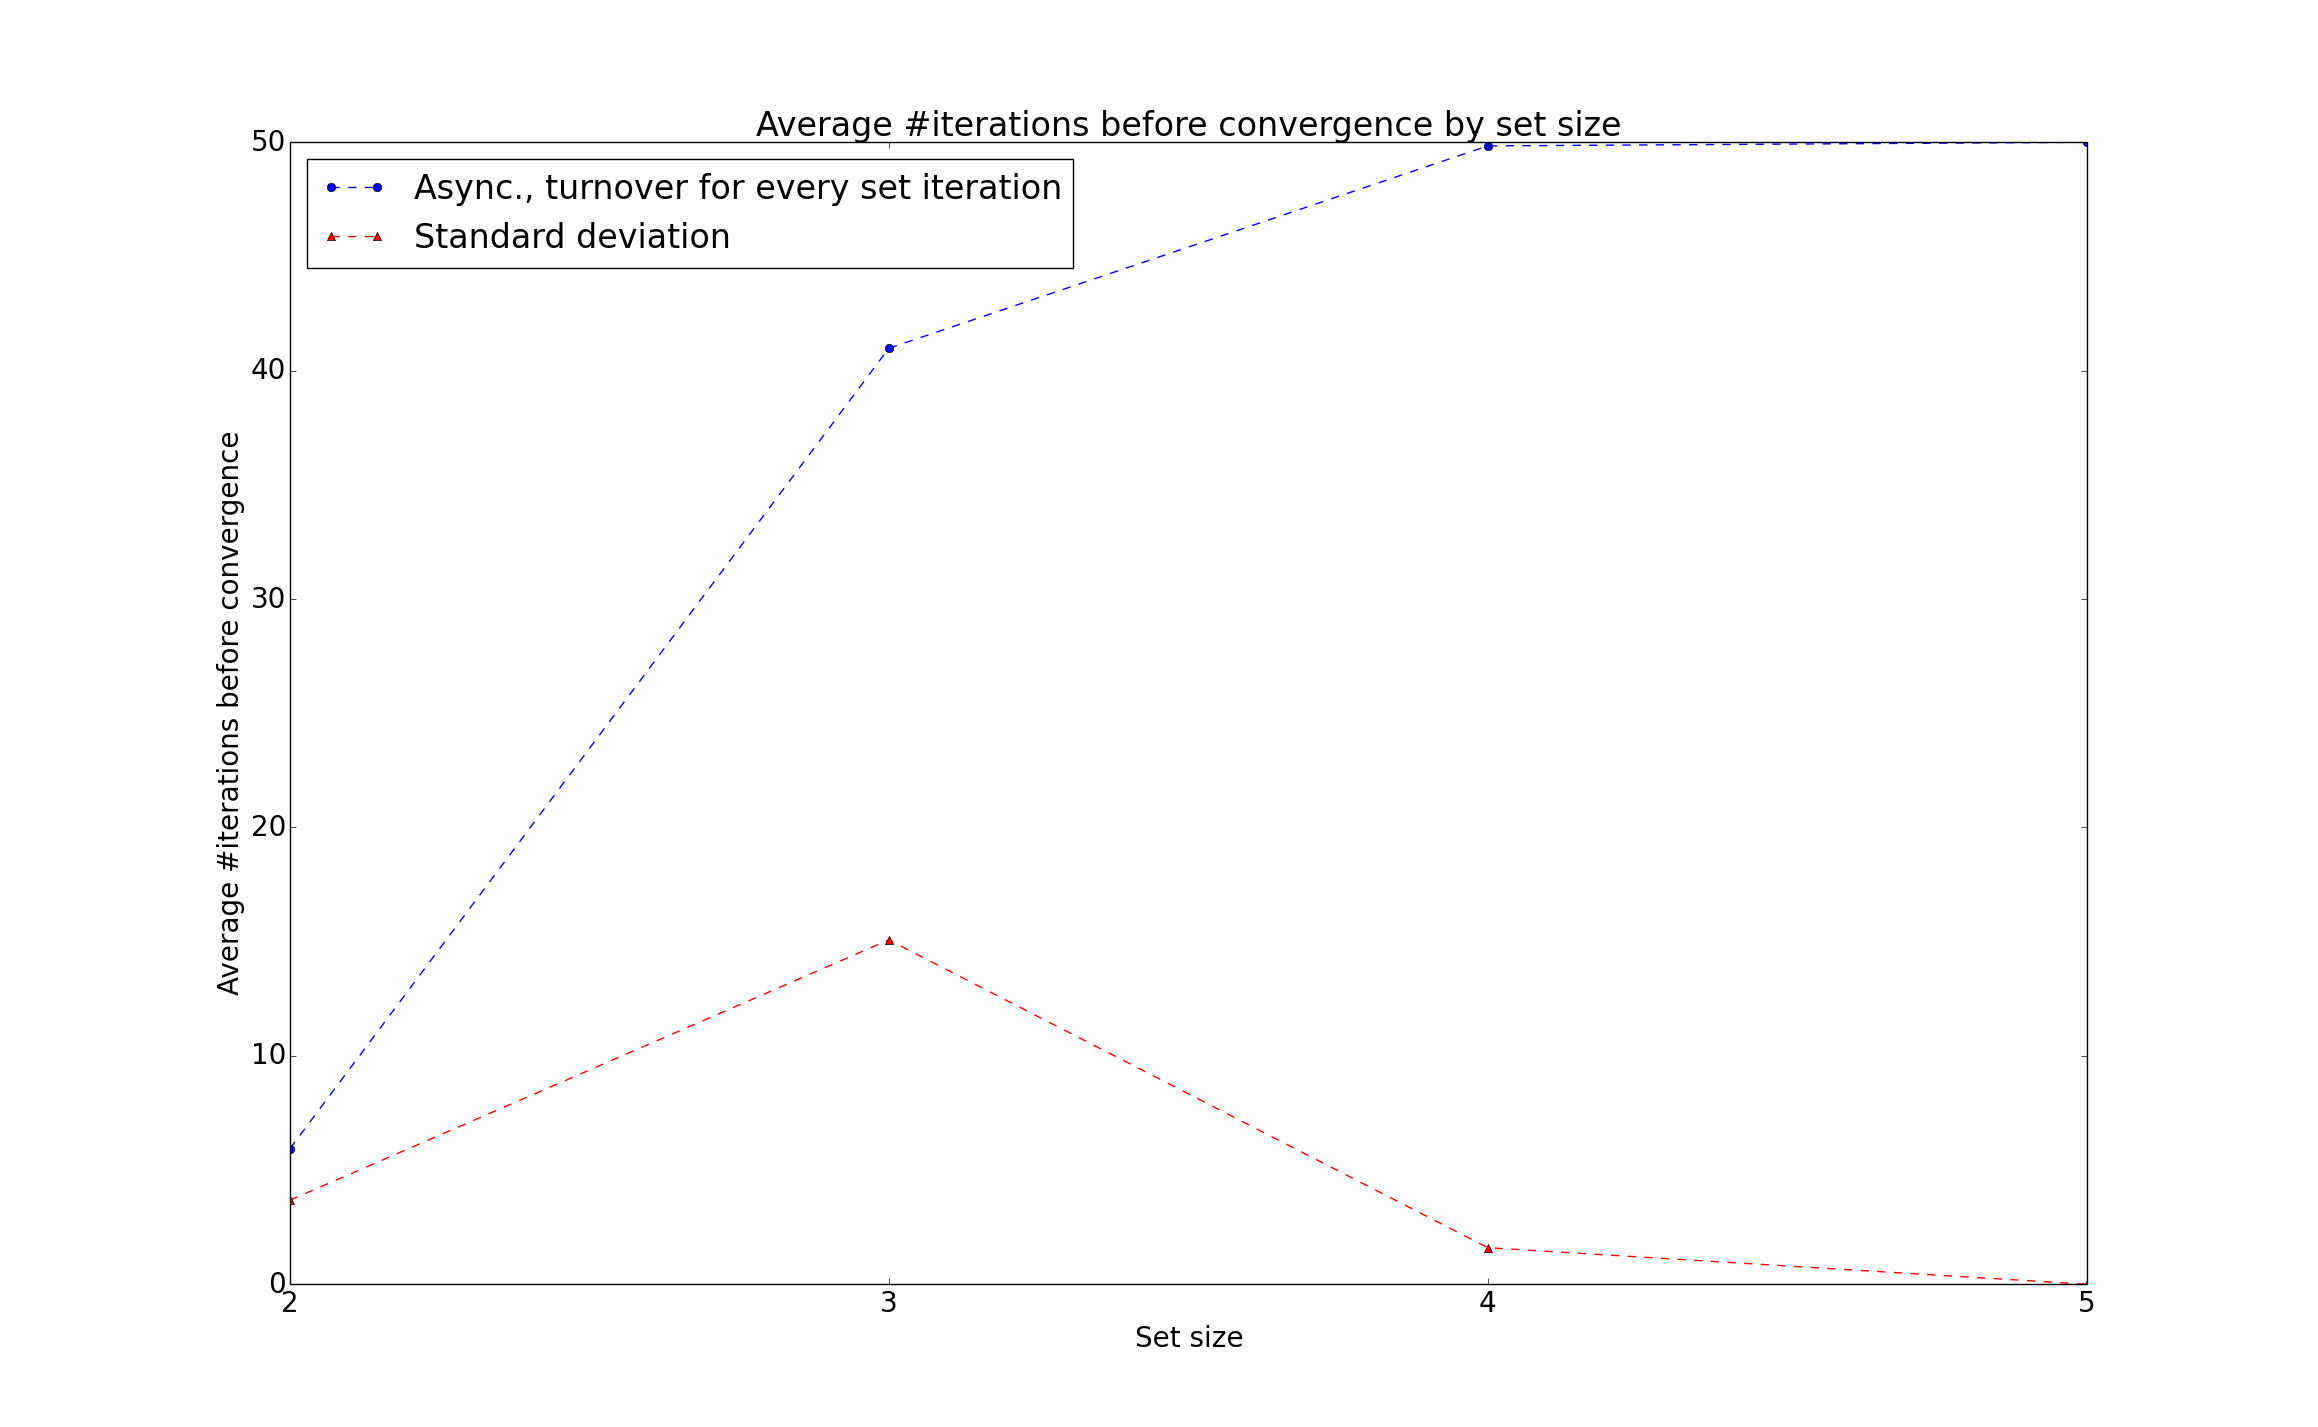
\includegraphics[width=13cm]{fig/avg_convergence_iterations_async_true_mode_1.png}
%     \caption{avg iters to convergence, most successful; async true mode 1}
%     \label{fig:avg_convergence_iterations_async_true_mode_1}
% \end{figure}

% \begin{figure}[h!]
%     \centering
%     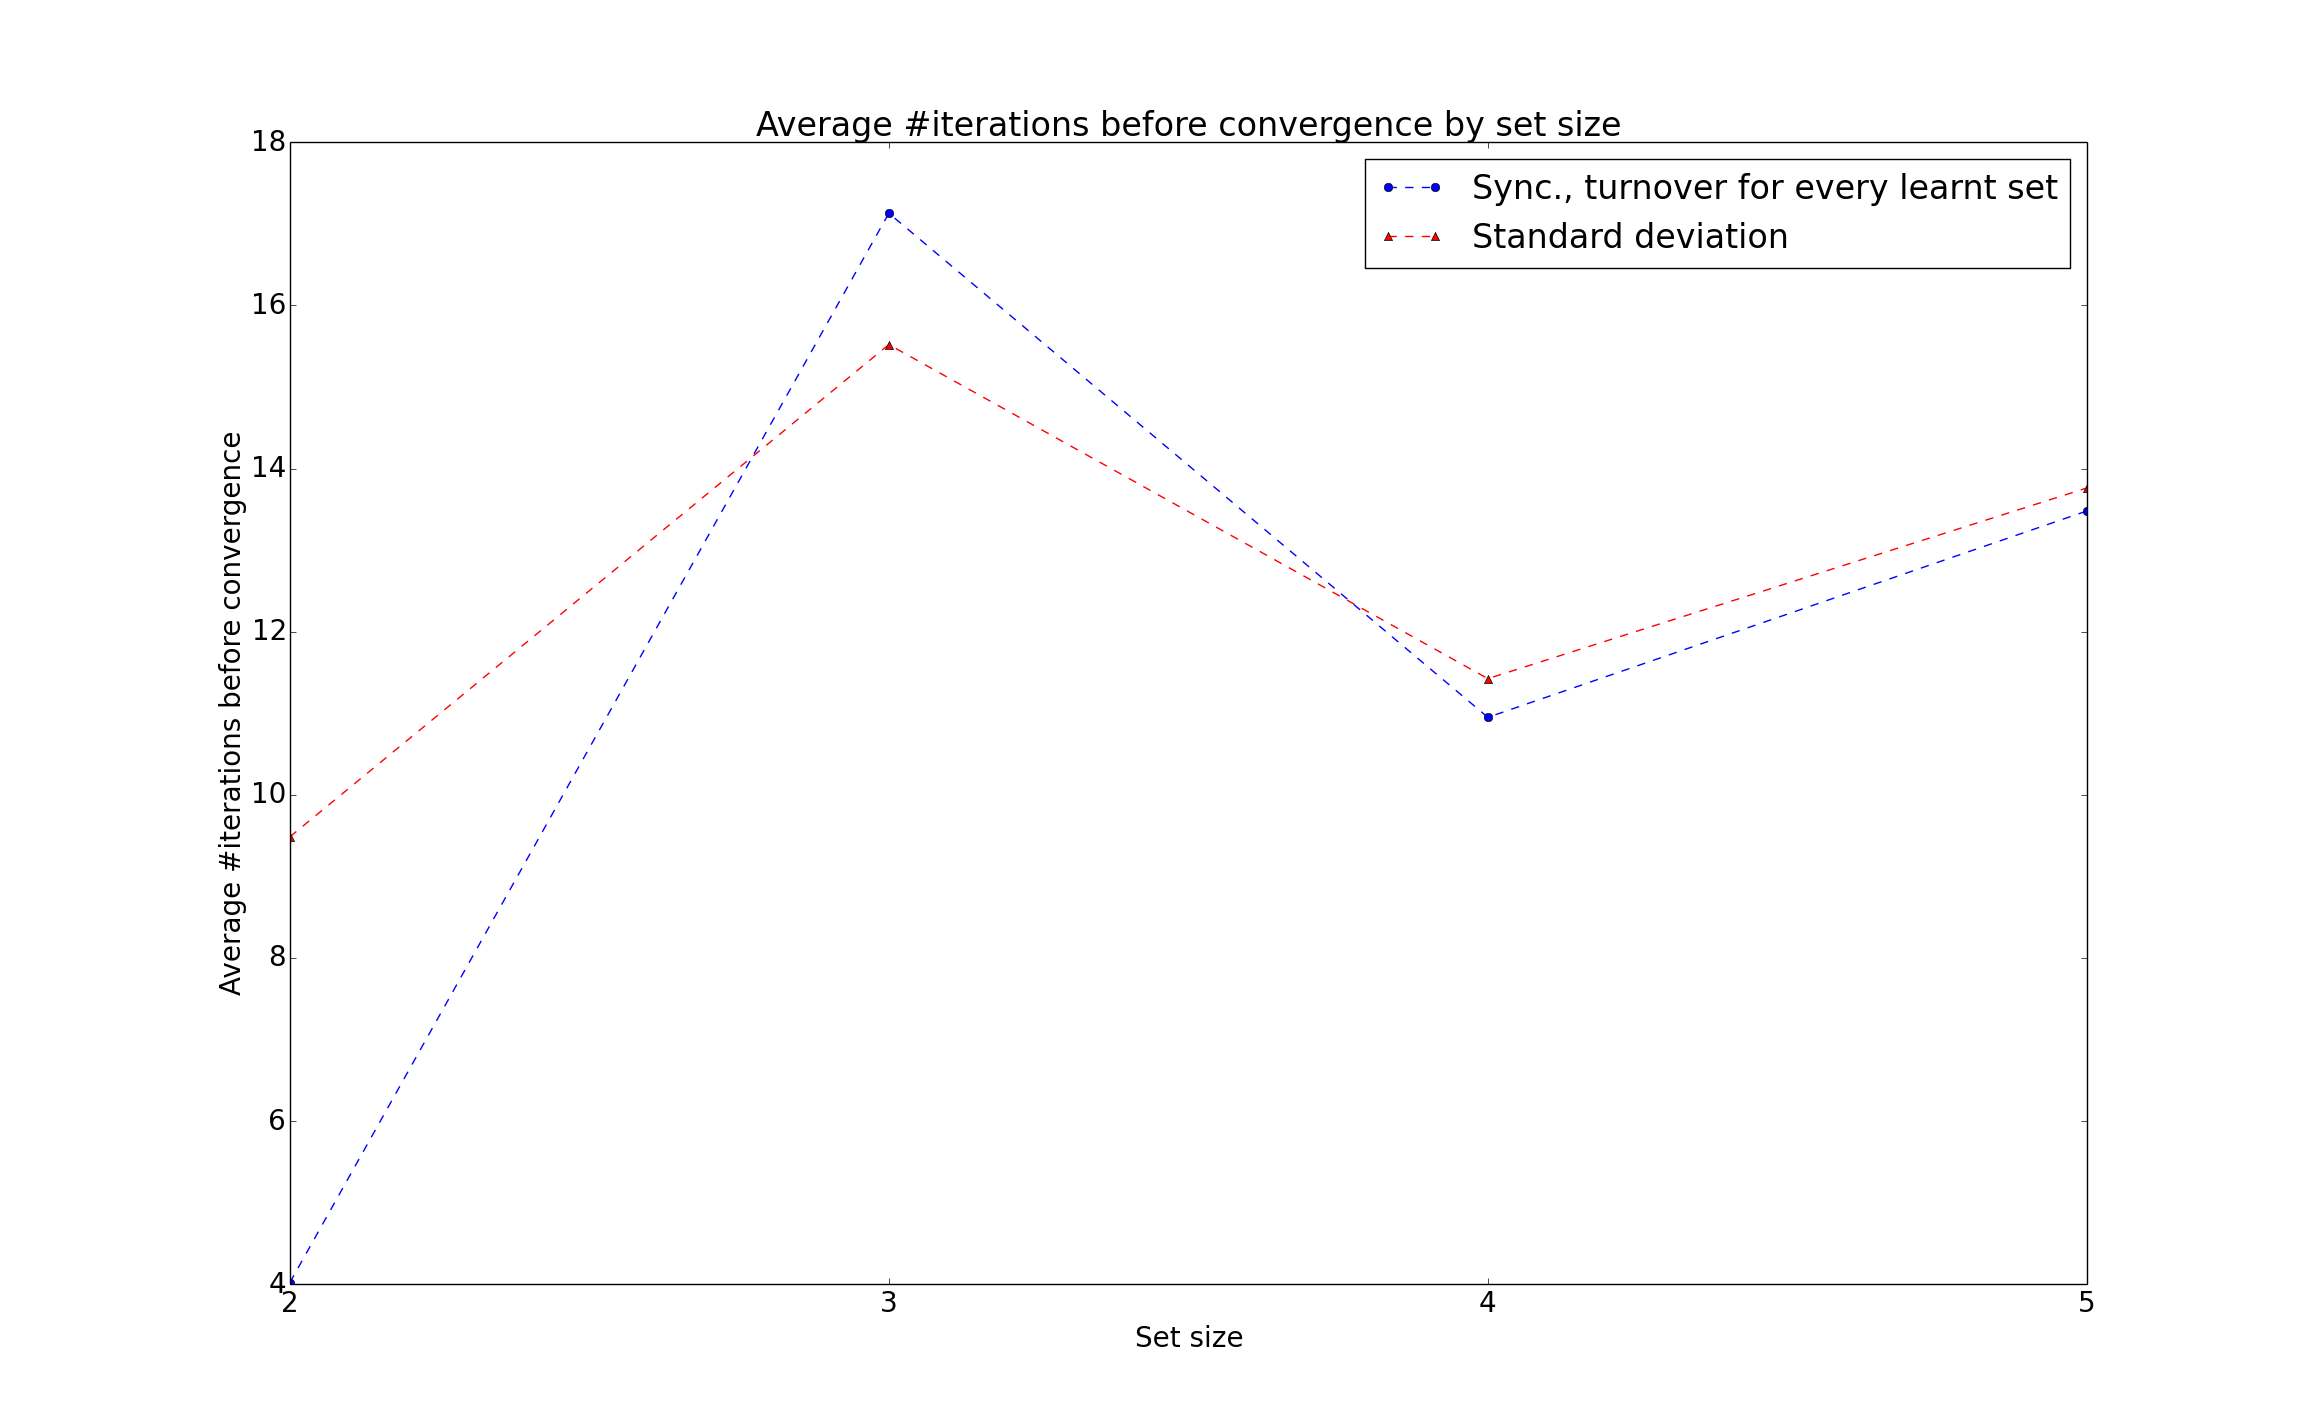
\includegraphics[width=13cm]{fig/avg_convergence_iterations_sync_mode_0.png}
%     \caption{avg iters to convergence, most successful; sync mode 0}
%     \label{fig:avg_convergence_iterations_sync_mode_0}
% \end{figure}

% \begin{figure}[h!]
%     \centering
%     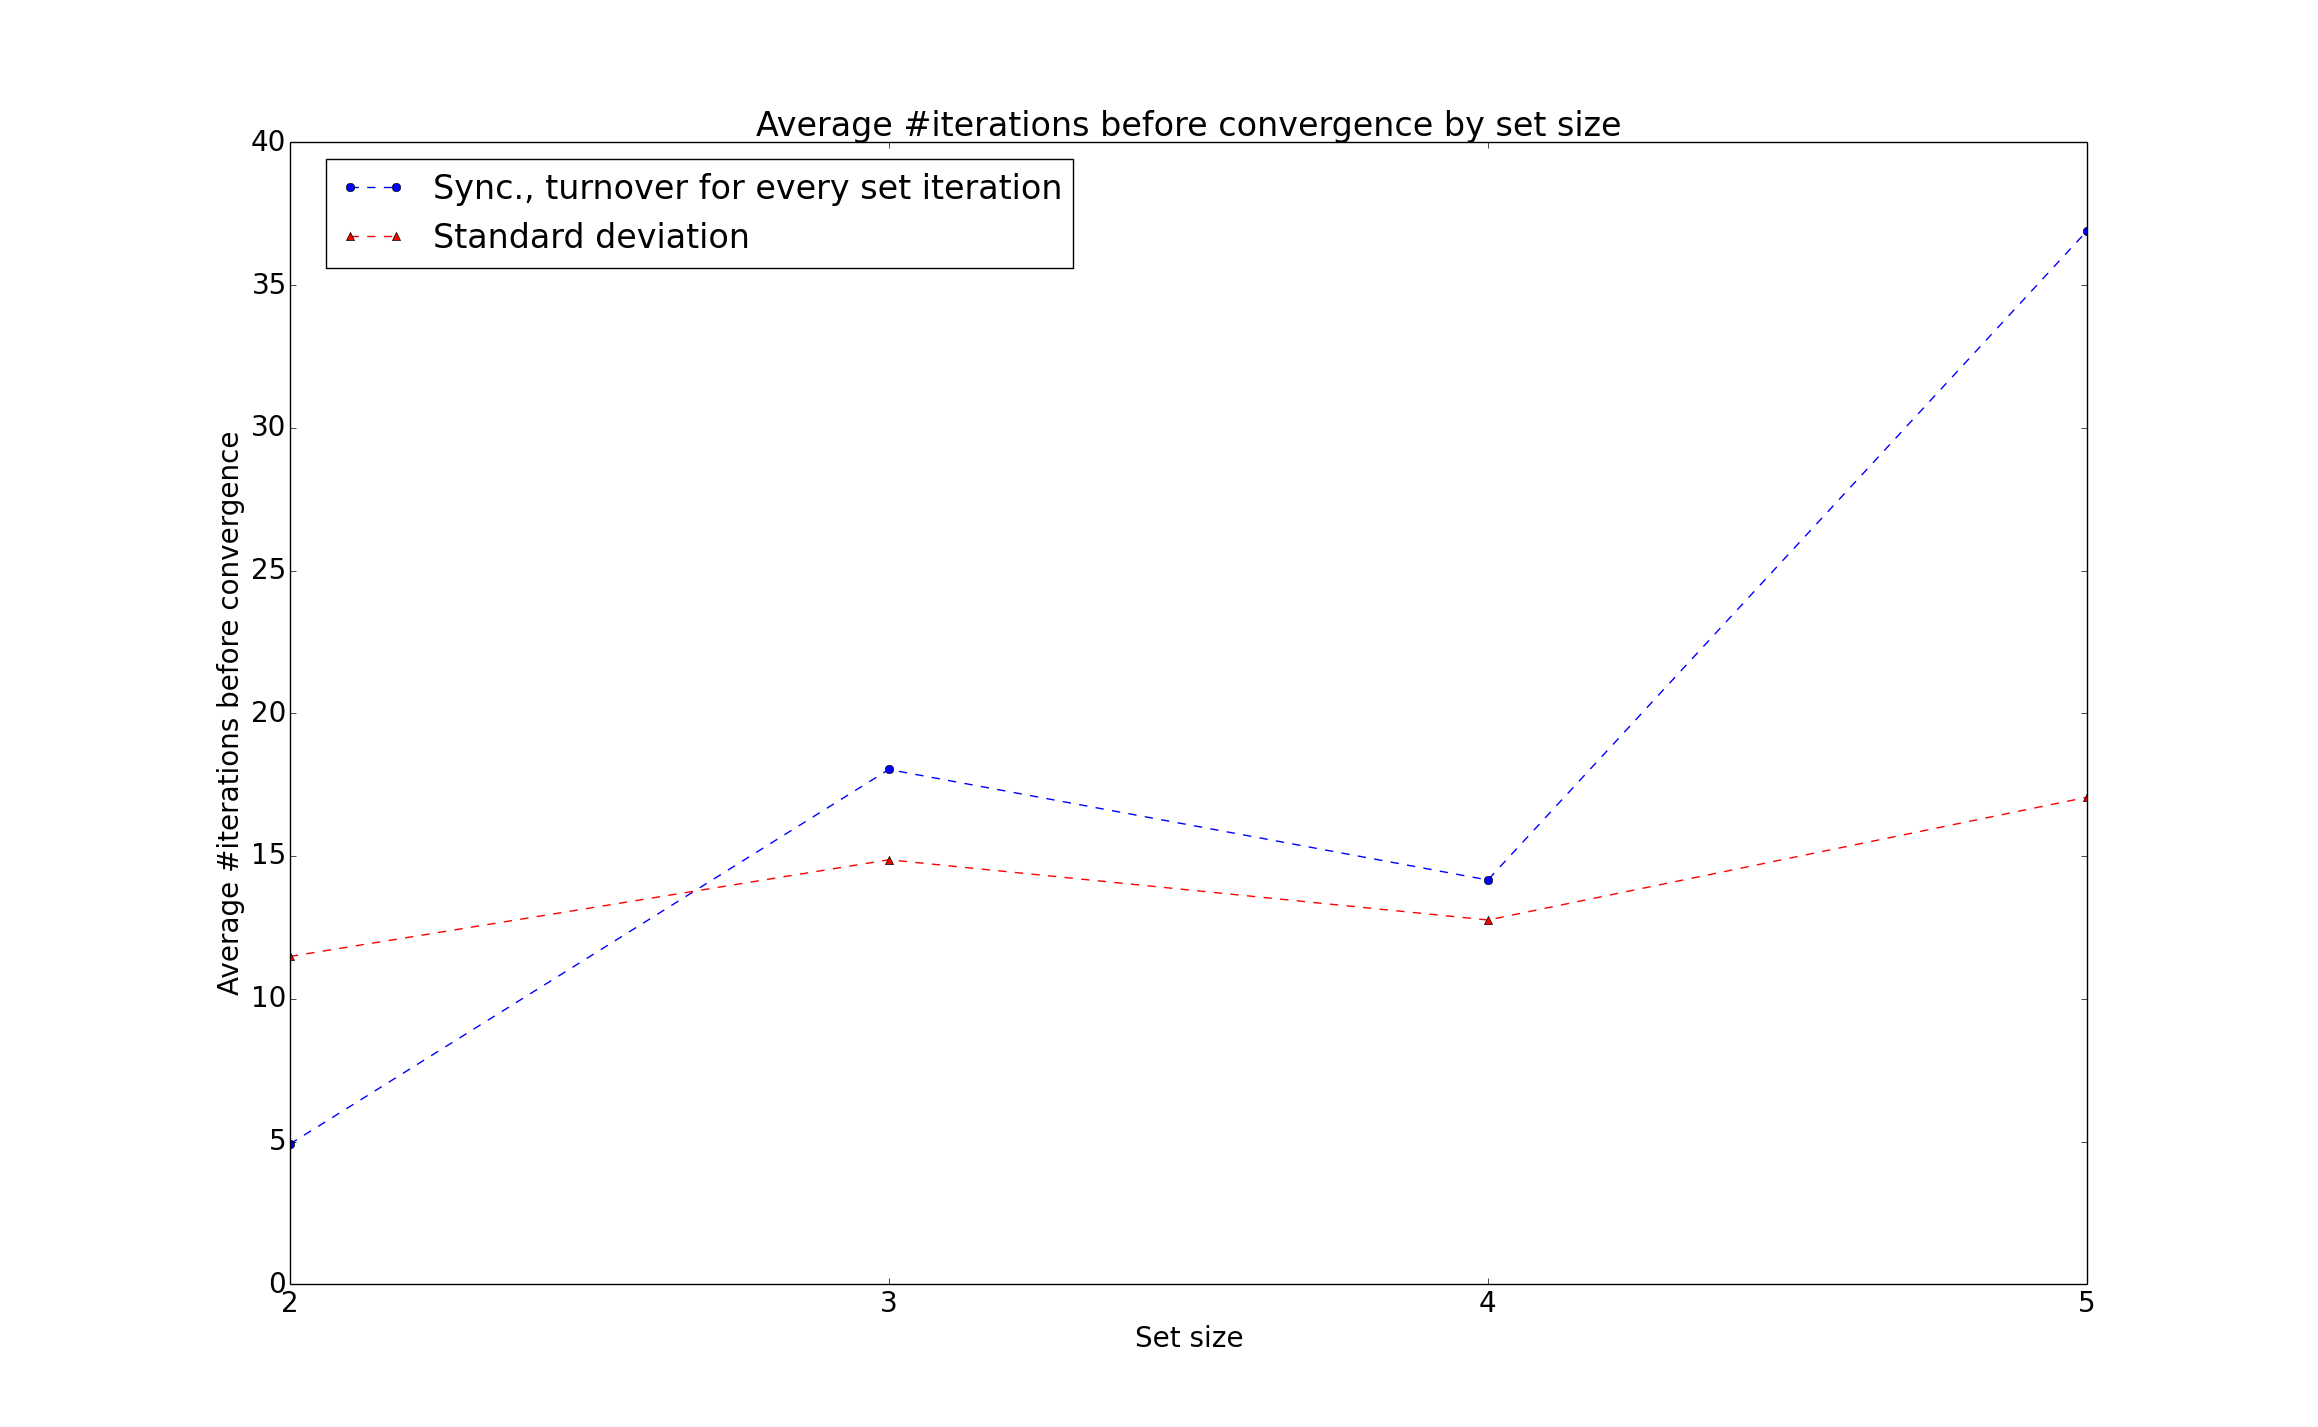
\includegraphics[width=13cm]{fig/avg_convergence_iterations_sync_mode_1.png}
%     \caption{avg iters to convergence, most successful; sync mode 1}
%     \label{fig:avg_convergence_iterations_sync_mode_1}
% \end{figure}

\begin{figure}[h!]
    \centering
    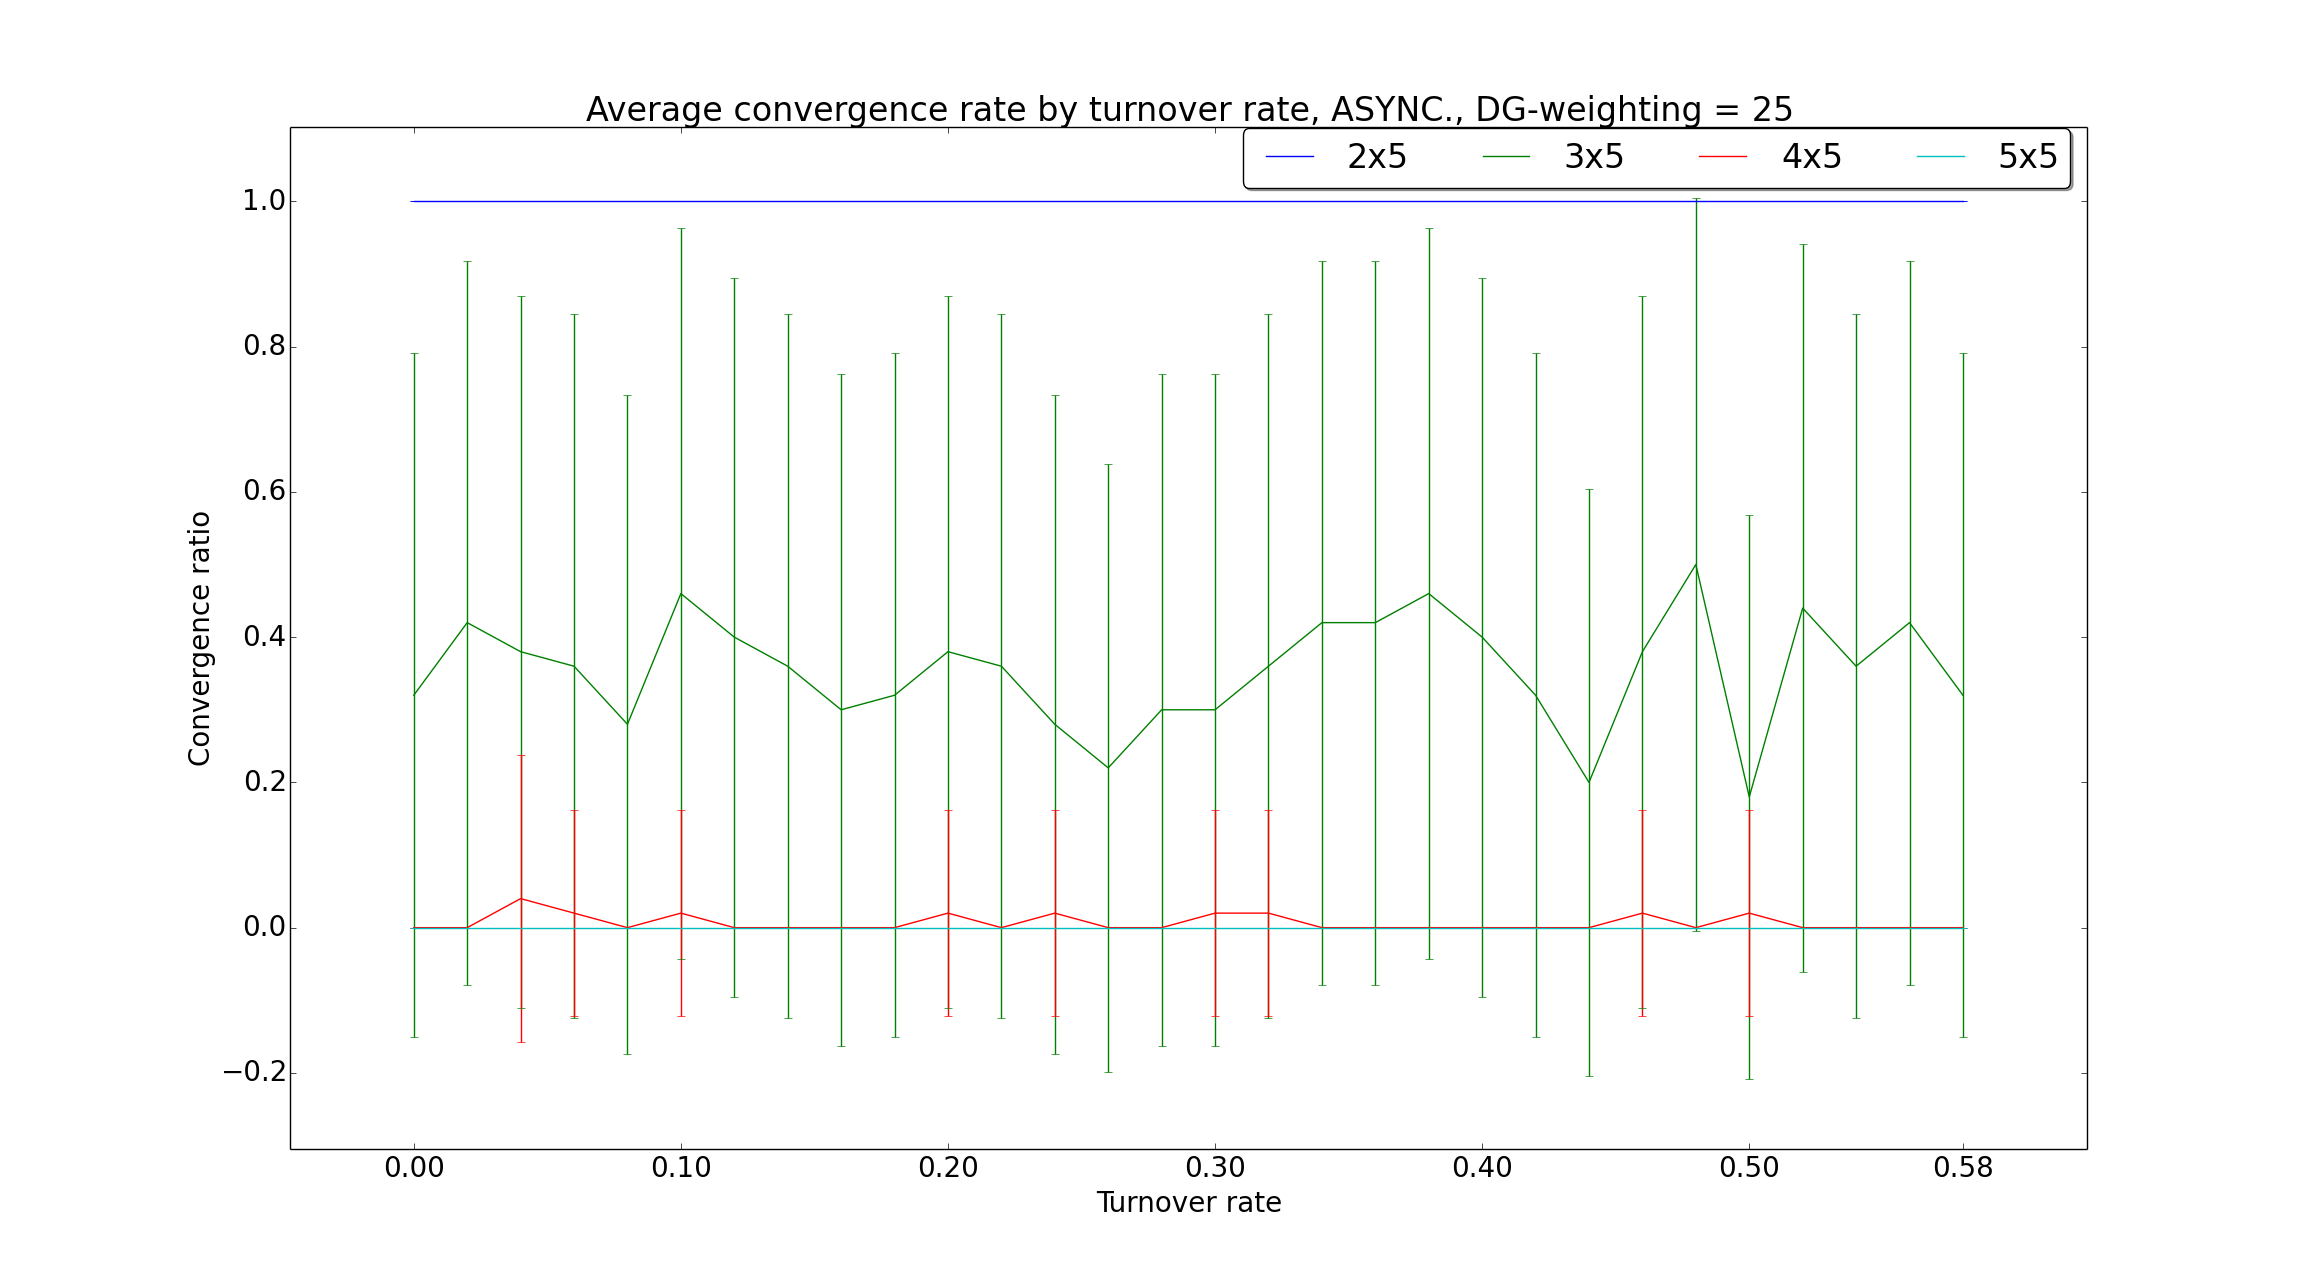
\includegraphics[width=14cm]{fig/avg_convergence_by_turnover_rate_async_dgw_25.png}
    \caption{avg convergence by turnover rate, async, dgw 25. note that it does not seem to impact this configuration - possibly async altogether. need to analyse changing the turnover rate for dgw 1, and also dgw for turnover rate 0.5 and 0.04}
    \label{fig:avg_convergence_by_turnover_rate_async_dgw_25}
\end{figure}

\begin{figure}[h!]
    \centering
    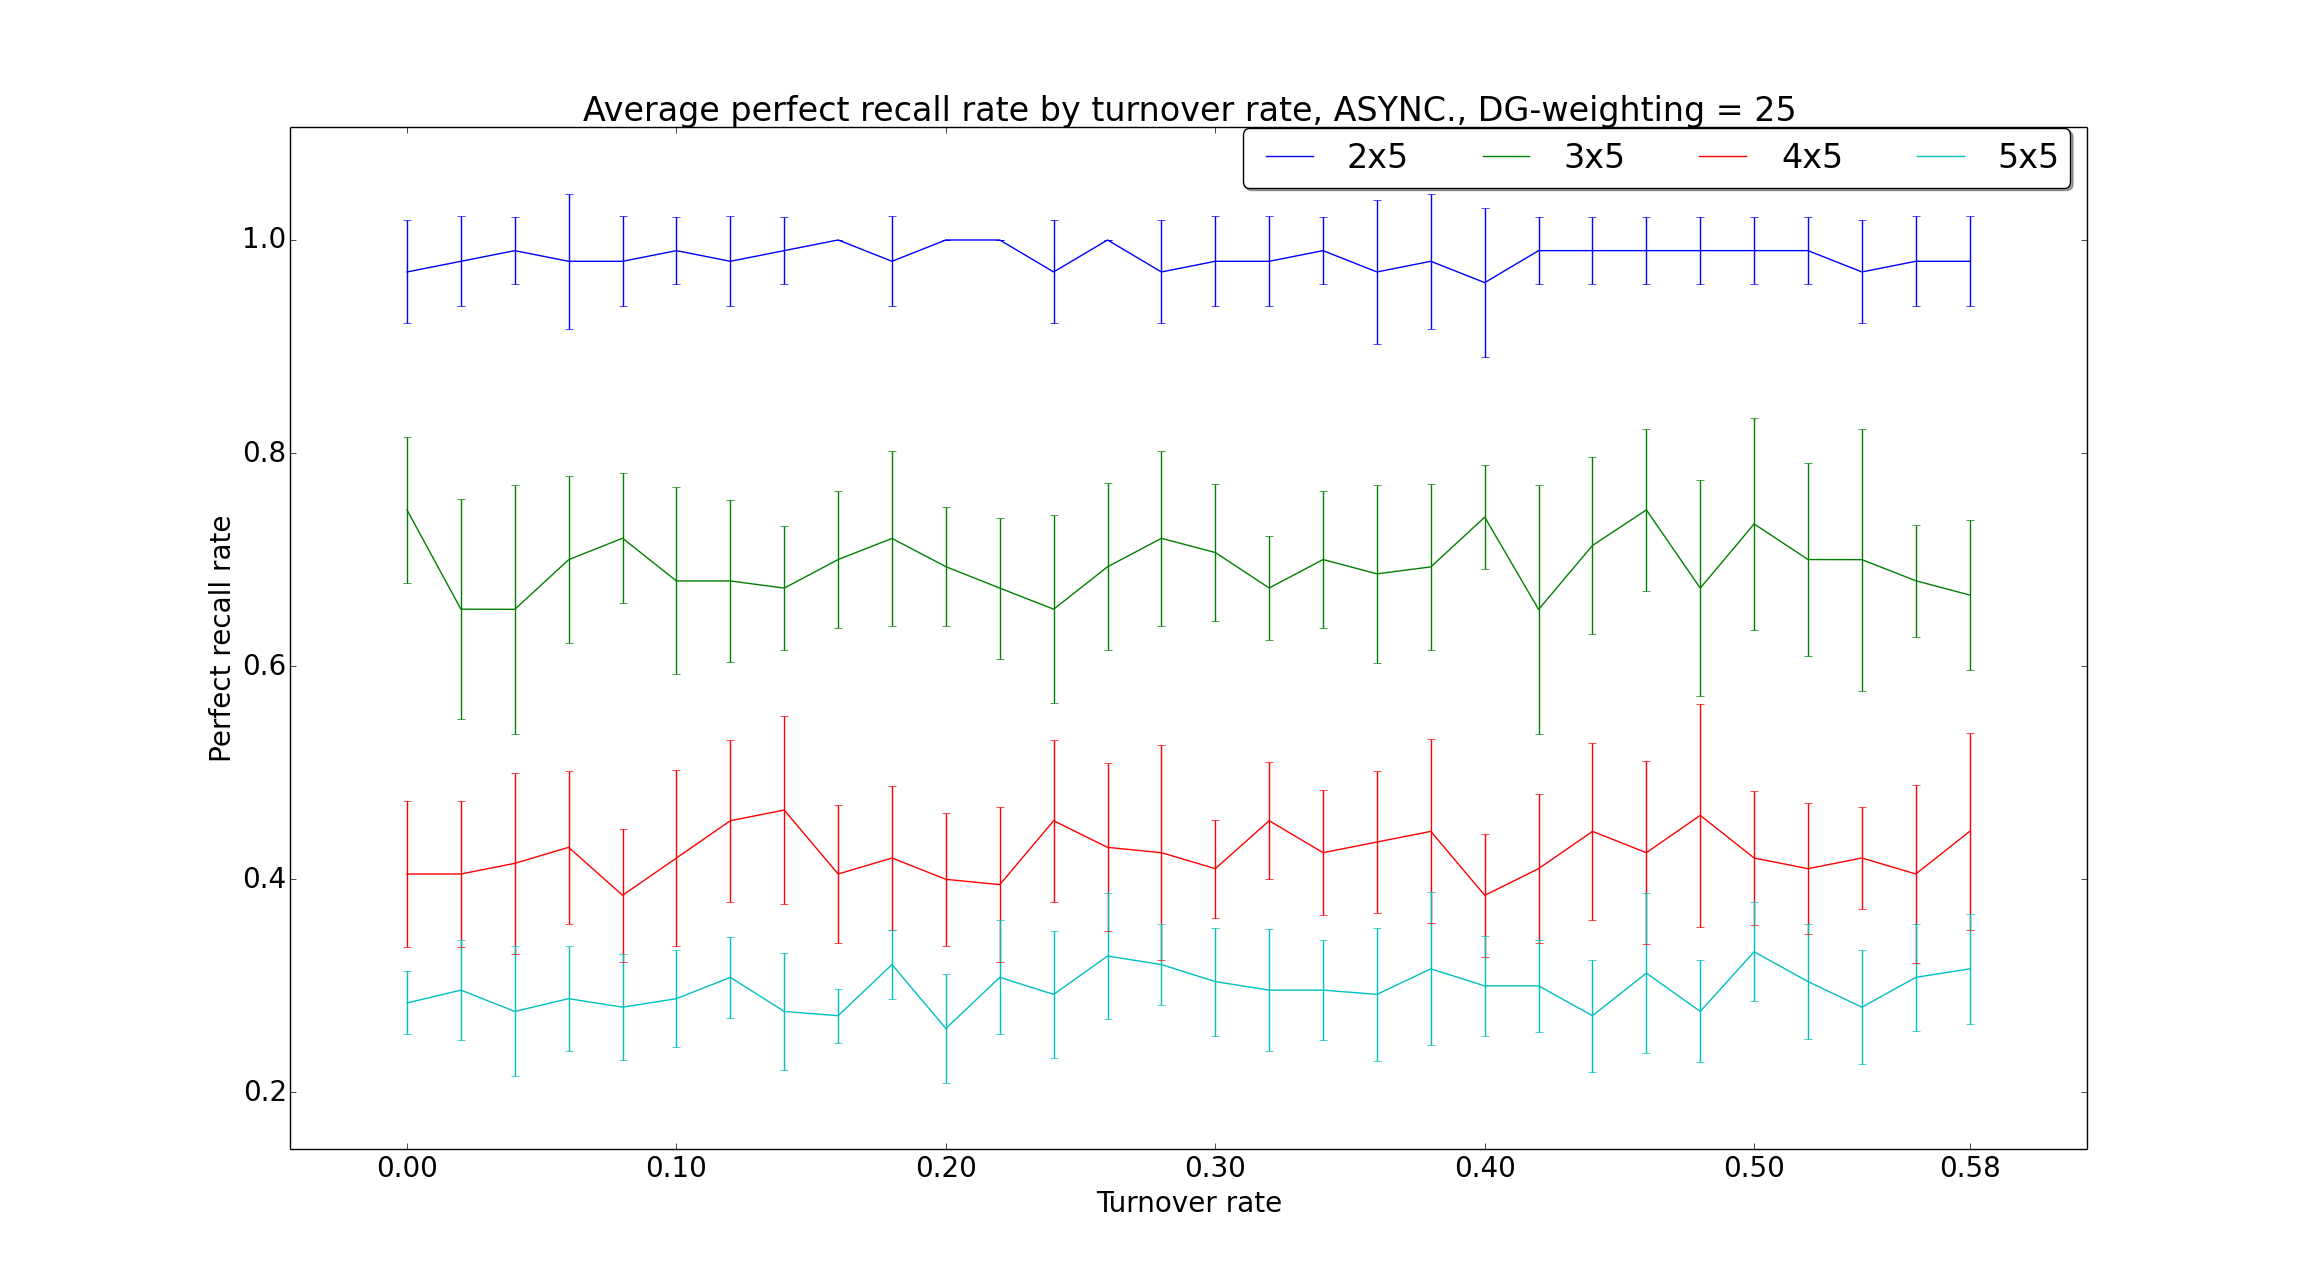
\includegraphics[width=14cm]{fig/avg_perfect_recall_rate_by_turnover_rate_async_dgw_25.png}
    \caption{avg perfect recall rate by turnover rate. note that it does not seem to impact the p.r.r. - see figure above. possibly async removes the impact this may have, although not successfully separating the given patterns - though increasing perfect recall for smaller set sizes when successful separation occurs.}
    \label{fig:avg_perfect_recall_rate_by_turnover_rate_async_dgw_25}
\end{figure}

\begin{figure}
    \centering
    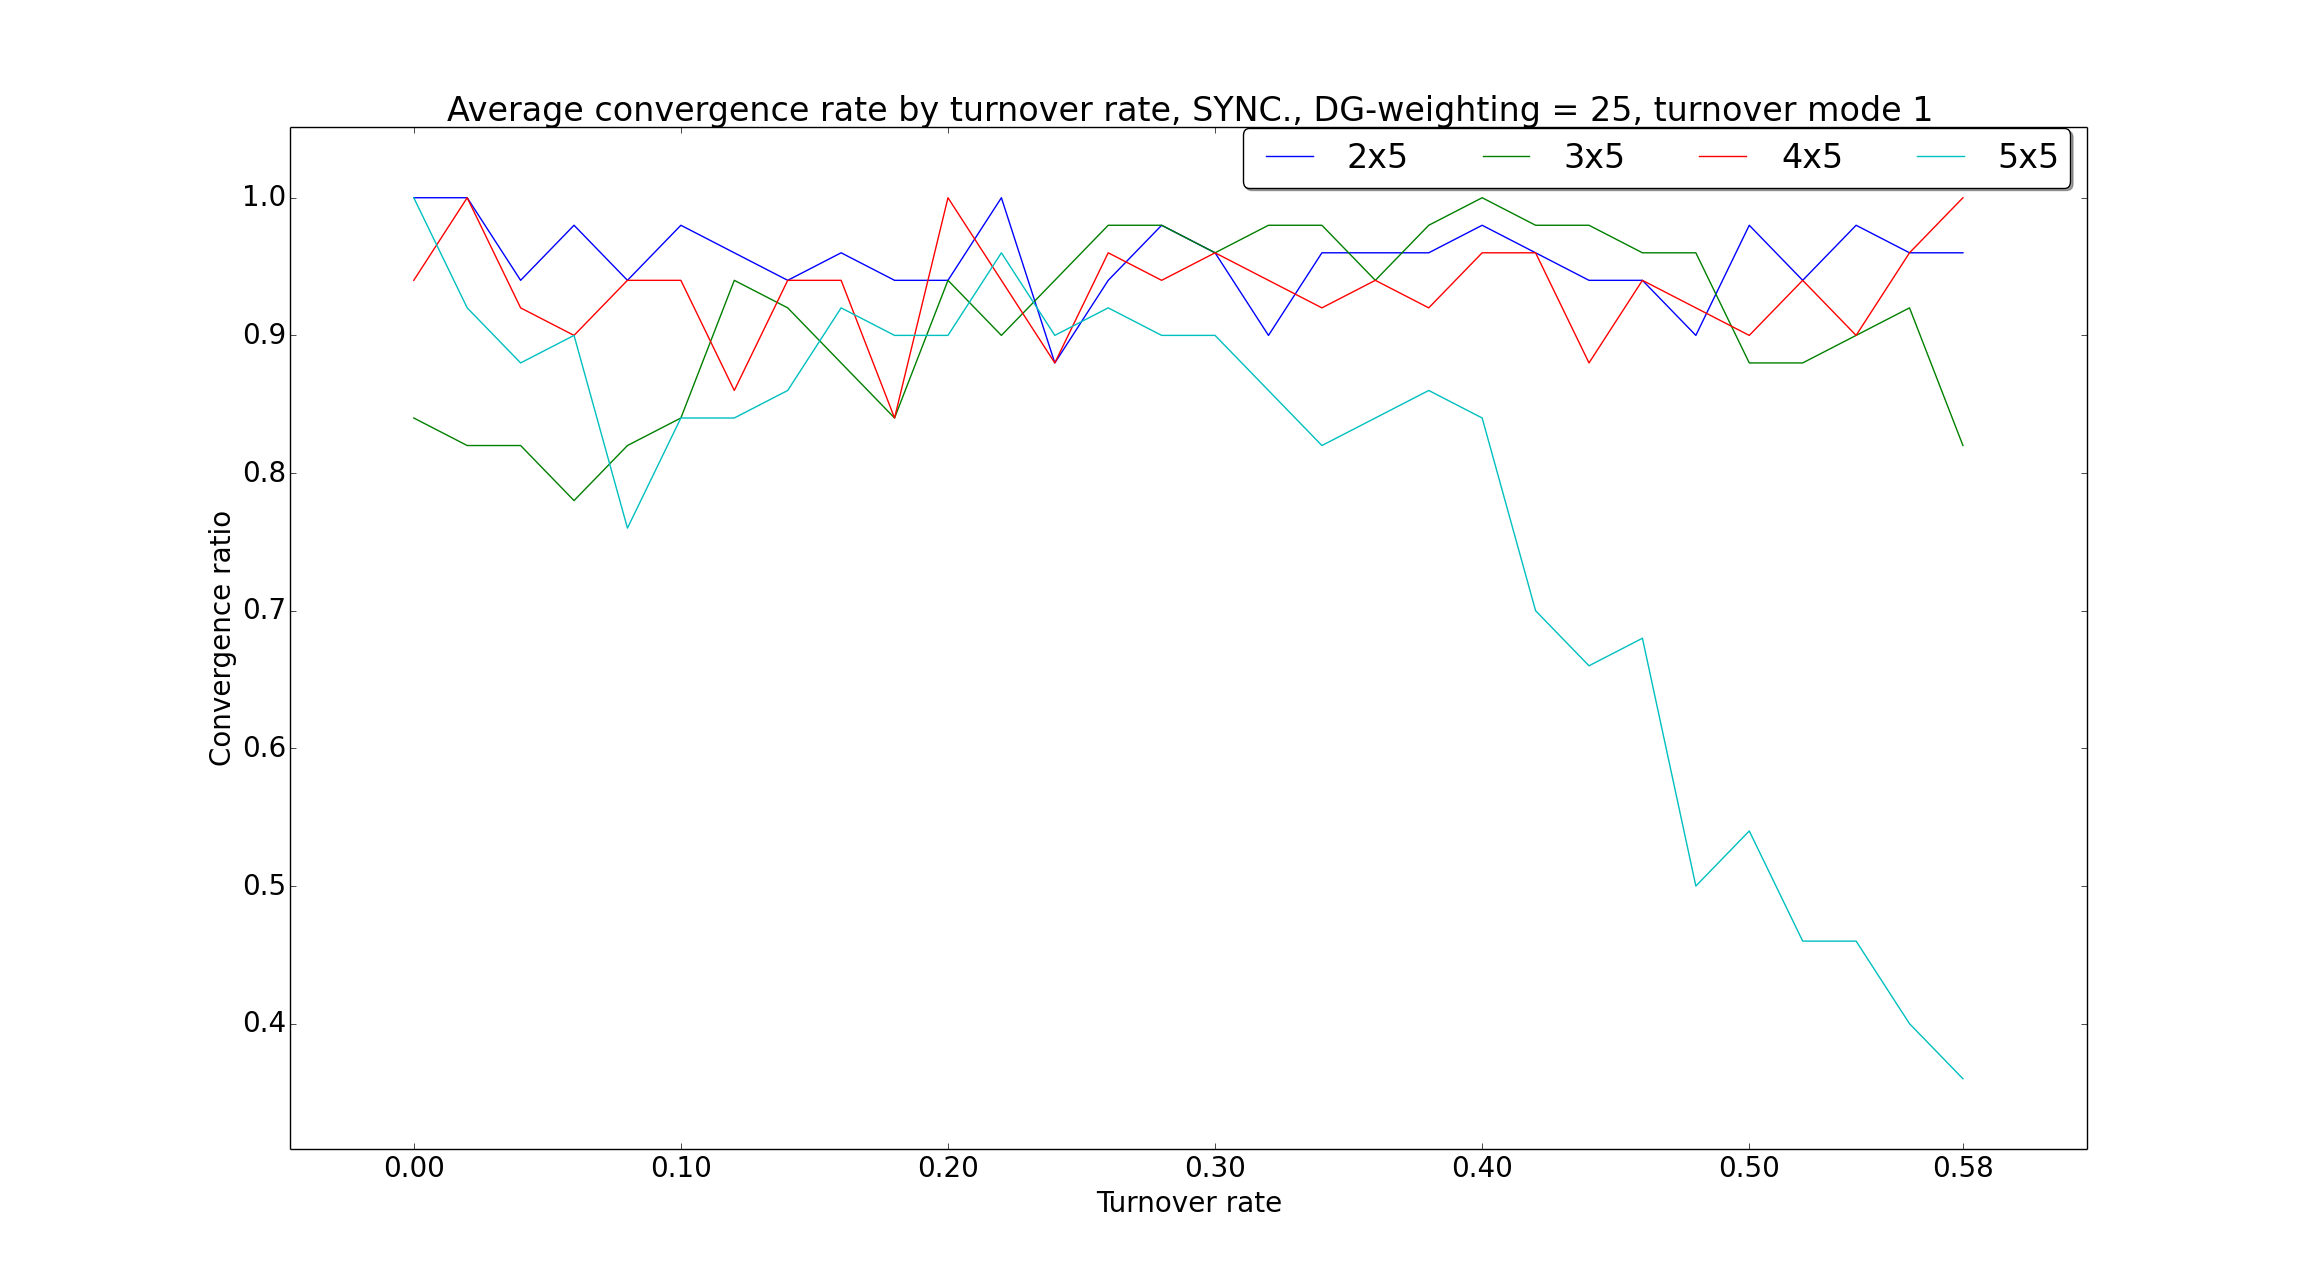
\includegraphics[width=14cm]{fig/avg_convergence_by_turnover_rate_sync_dgw_25_t_m_1_no_err_bars}
    \caption{avg convergence by turnover rate. updating scheme ca3: synchronised. dentate gyrus weighting: 25, turnover mode: 1, i.e. turnover for every new set. no err bars}
    \label{fig:avg_convergence_by_turnover_rate_sync_dgw_25_t_m_1_no_err_bars}
\end{figure}

\begin{figure}
    \centering
    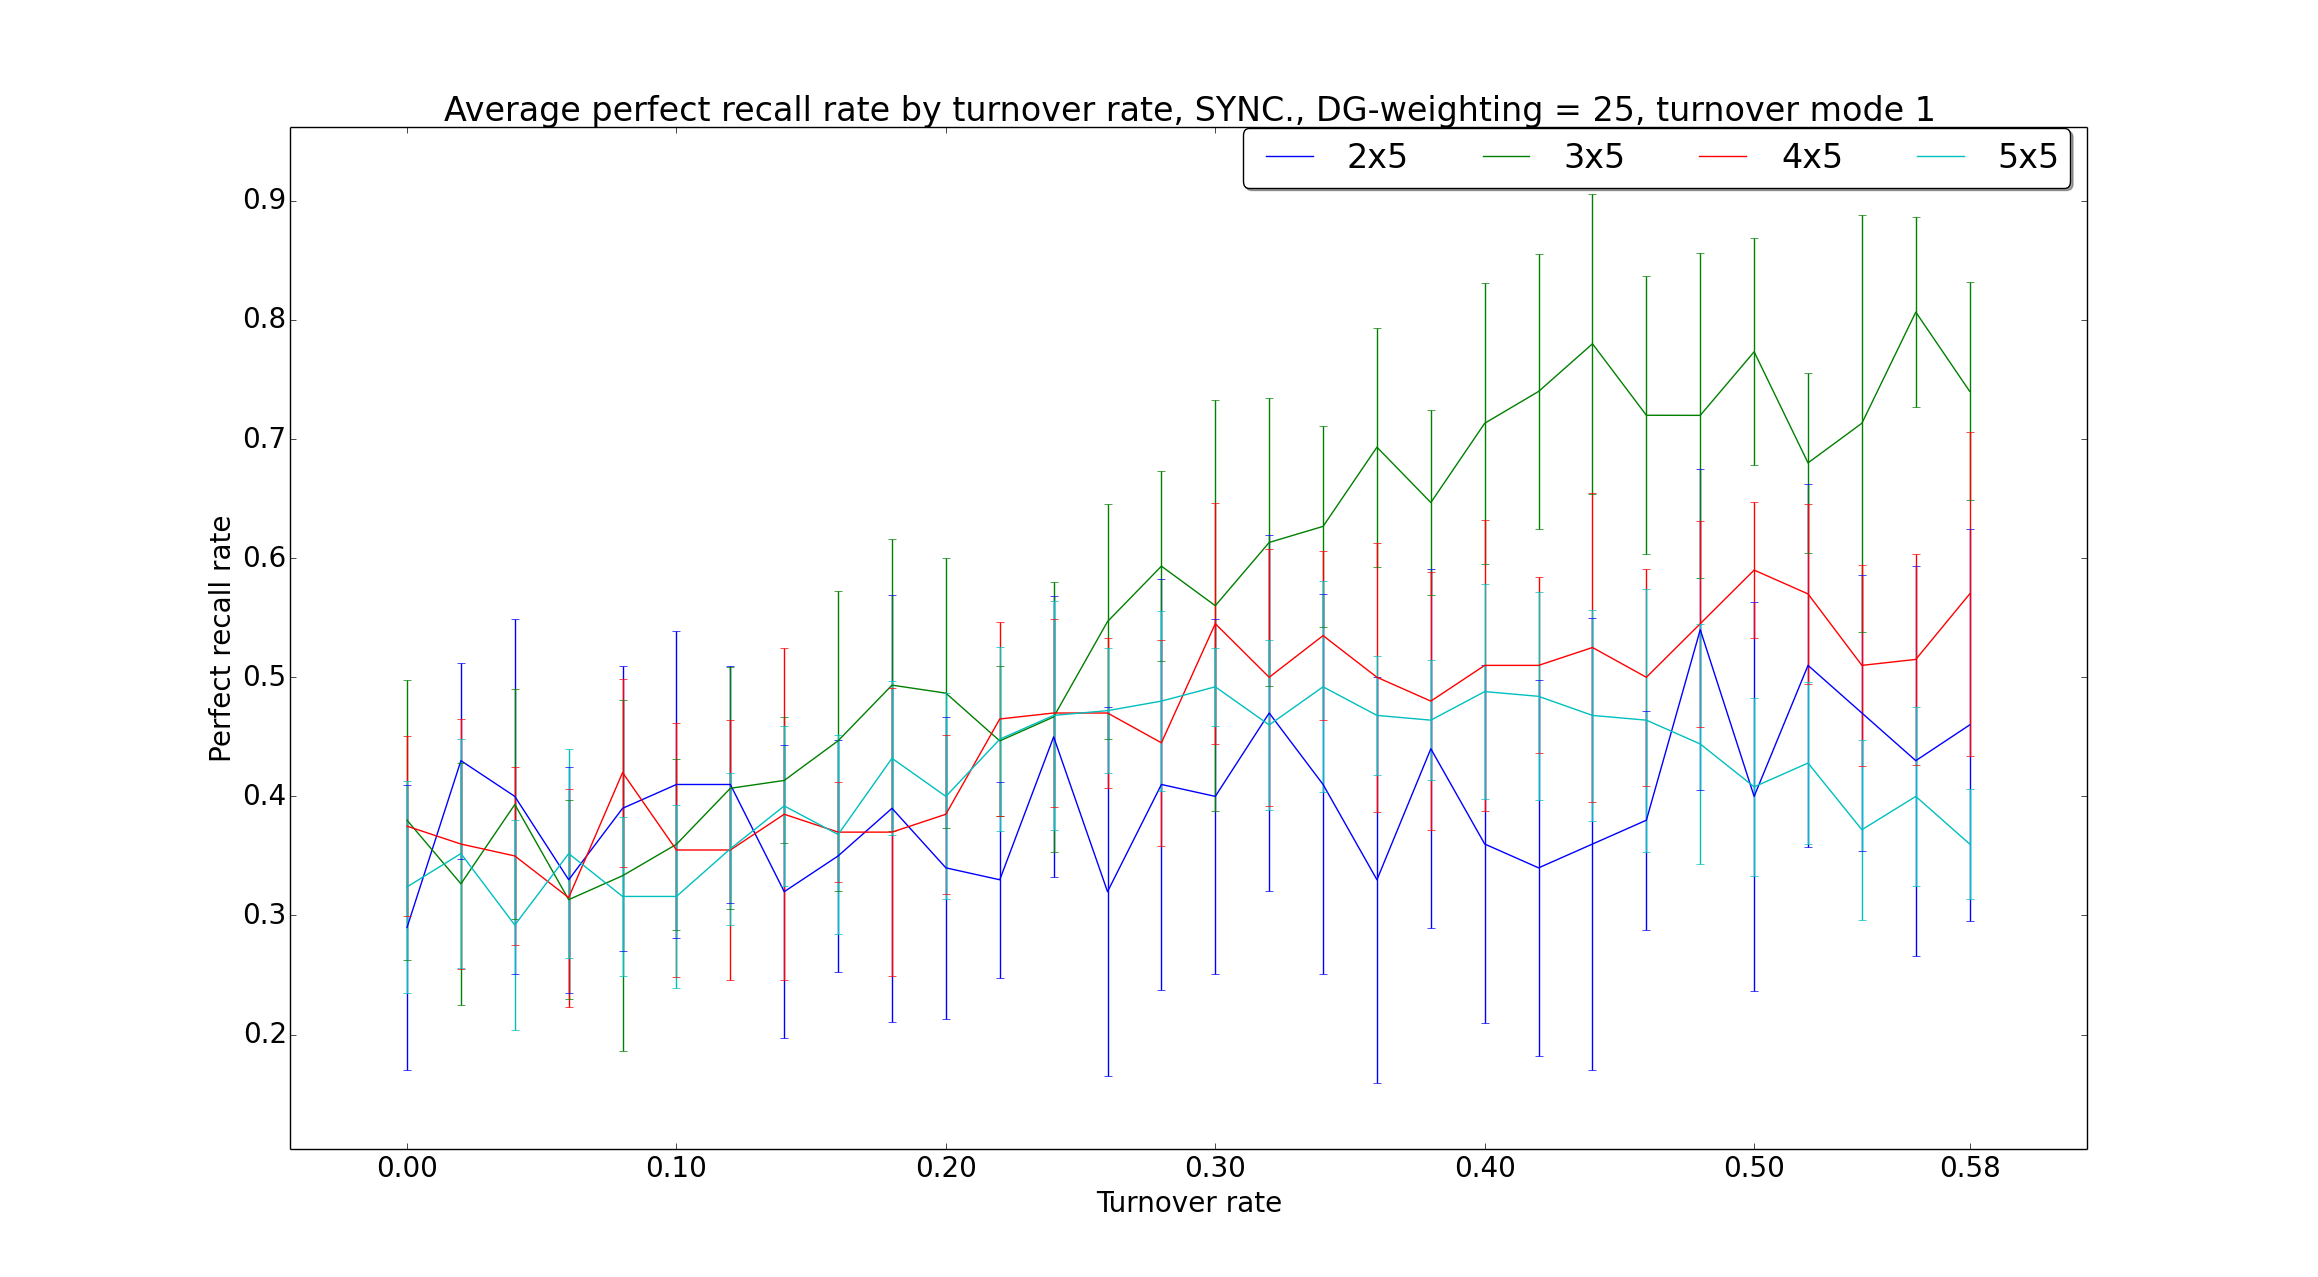
\includegraphics[width=14cm]{fig/average_perfect_recall_rates_by_set_size_sync_dgw_25_t_m_1}
    \caption{avg perfect recall rate by turnover rate. updating scheme ca3: synchronised. dentate gyrus weighting: 25, turnover mode: 1, i.e. turnover for every new set. no err bars}
    \label{fig:average_perfect_recall_rates_by_set_size_sync_dgw_25_t_m_1}
\end{figure}

\subsection{Experiment 2: Hippocampal model calibration}
\subsubsection{Methods}
\subsubsection{Results}

\subsection{Experiment 3: Extracting auto-associative patterns by chaotic recall}
\subsection{Experiment 4: Extracting hetero-associative patterns by chaotic recall}

\subsection{Experiment 5: Consolidation performance, experiment 3}
\subsection{Experiment 6: Consolidation performance, experiment 4}

\subsection{Experiment Y: Novel}

some patterns may be recalled after the next training set has been learned. i allowed this to put the pattern in the set of chaotically recalled patterns, because it reflects something which is fairly stable in the hippocampal module.
\\

Async. seems to be by far the most accurate in terms of perfect recall when it converges. Sync. with turnover for every learnt set has the highest convergence rate - non-changing for different set sizes, but the worst perfect recall rate.

It would be very interesting to see how using the 'spurious' patterns along with the actual matching patterns would consolidate to the neocortical network, comparing this to the performance attained by using the formerly outlined pseudopattern generation. In the event of having a similar effect from pattern consolidation using spurious patterns, this may point in the direction of spontaneously generated 'spurious' patterns in fact possibly acting as pseudopatterns, thus outlining a process for pseudopattern generation in the brain. (Where the stability during recall could determine the consolidation strength. For complete convergence during training using async, mode 0, about 7 iterations were required for convergence - which is thought to be (?) the number of required iterations for successful neocortical memory consolidation. This could be a spurious correlation - however, the number is equal during convergence for set size 2. If the same number of iteration can be required for a successful configuration for set size 3, this would suggest that the number is not spurious.)
\\

Along with the spurious patterns, if considering the sum of distinct perfectly recalled patterns and spurious patterns as containing information about the number of patterns, the asynchronous scheme seems to contain the most information, only falling off at set size 5. This is most likely due to the convergence being 0 \% , which it actually is at set size 4, too. Increasing the number of iterations may remedy this - however, a further calibration is most likely more relevant.
\\

The recall rate is much better for the same convergence rate in the asynchronous scheme, which points towards this being the preferable scheme. Furthermore, because turnover for every set iteration remains biologically implausible, a more plausible, yet still unrealistic model should be chosen. I.e. Async., turnover for every new set.

STD only log() in async. -> points to more stable/realistic mechanism?
\\

Gradual exposure through the constant output of the HPC during recall and learning? If this may consolidate something to the PFC, it would be really interesting.
\\

In order to target the black-box analysis that analyzing an ANN can be - particularly for the case of biologically realistic networks using chaotic neurons - I employed a type of logging, from which data is parsed, and sorted by a parser that I wrote. This data includes the number of spurious patterns extracted, where spurious is defined as not perfectly overlapping any of the provided training patterns. Furthermore, it includes the number of iterations before convergence, where 50 iterations is considered as failure to converge. It also includes the weighting selected for the connections from the DG, the neuronal turnover rate that was employed, and lastly the number of extracted patterns, along with the perfect recall rate for the current experiment.
\\

appears to be a significant correlation between the convergence rate and the perfect recall rate. this probably correlates with most positive emergent attributes that we wish to attain in the HPC network


% \begin{figure}
% \centering
% \includegraphics{fig/}
% \caption{Caption}
% \label{fig:my_label}
% \end{figure}


% ========================== section ============================
Experiment design
Results
Comparisons

\section*{Notes}

Enforce sparsity through weight updates corresponding only to the winners of kWTA - didn't work.

\textbf{100 \% connection ratio EC-CA3:}

Fairly rapid convergence for three patterns in HPC-module for turnover between every training set iteration. 
Not necessarily successful recall of all patterns. Does this have something to do with the synchronized CA3-layer during recall? Separation possible during recall when the desired pattern(s) are presented to the network - however, not all may be recalled.

-> New random pattern each time stability was reached resulted in better recall.

Is this also the case for heavier weighting of the DG-CA3 path during learning?

Spurious pattern reduction/correlation with occurrence when using turnover?

Convergence when turnover is removed between set iterations?

Heavier weighting DG. Based on paper \citep{Norman2003}. Empirical results. Chpt. 4. Figures. Nice.

\section*{Model calibration}

Experiments designed for model calibration

Dimensions analyzed outlined above.

First: STM-network extraction rate (at first, empirically observed to be same as solely auto-associative Hopfield network).


\textbf{Notes}

experiments suite - two as outlined by \citep{Hattori2014}, originally retrieved from ... as outlined above
enabling several trials automatically.

Turnover between every training set iteration (?). Needs to include empirical data on decision making. Move to preliminary experimentation in chpt. 4?
\\

It would be interesting to see HPC expanded to include neo. nets activity fed back into the hpc net. in order to induce activity. Perhaps this may cycle through previous patterns. Expanding the model towards Wakagi (08), and using a kind of reverberation could be a focal point in future work.


\cleardoublepage